% =====================================================================
%  第 2 章 路径积分形式 —— ch02c（§2.8）
%  页段：PDF 139–161（原书 p.138–160）
% =====================================================================

% 四指标配对图：参数为若干对数，如 {0/1,2/3}；无参数则四个指标都不配对
\newcommand{\wickfour}[1]{%
\begin{tikzpicture}[baseline=-0.6ex,x=0.42cm,y=0.28cm]
  \foreach \xx/\ll in {0/{$i$},1/{$j$},2/{$k$},3/{$l$}}{
    \fill (\xx,0) circle (1.1pt);
    \node[above,inner sep=1.2pt,font=\scriptsize] at (\xx,0.08) {\ll};}
  \foreach \aa/\bb in {#1}{%
    \draw[line width=0.5pt] (\aa,-0.06)
      .. controls (\aa+0.18,-0.52) and (\bb-0.18,-0.52) .. (\bb,-0.06);}
\end{tikzpicture}}

% 三价顶点：i 在上、j 在左下、k 在右下
\newcommand{\trivertex}{%
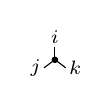
\begin{tikzpicture}[baseline=-0.5ex,x=0.30cm,y=0.30cm]
  \fill (0,0) circle (1.2pt);
  \draw (0,0.06)--(0,0.56)
    node[above,inner sep=1pt,font=\scriptsize] {$i$};
  \draw (-0.05,-0.03)--(-0.46,-0.34)
    node[left,inner sep=1pt,font=\scriptsize] {$j$};
  \draw (0.05,-0.03)--(0.46,-0.34)
    node[right,inner sep=1pt,font=\scriptsize] {$k$};
\end{tikzpicture}}

% 一条边：两端点 i 与 j
\newcommand{\edgeij}{%
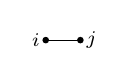
\begin{tikzpicture}[baseline=-0.5ex,x=0.44cm,y=0.30cm]
  \fill (0,0) circle (1.2pt);
  \fill (1,0) circle (1.2pt);
  \draw (0,0)--(1,0);
  \node[left,inner sep=1.5pt,font=\scriptsize] at (-0.04,0) {$i$};
  \node[right,inner sep=1.5pt,font=\scriptsize] at (1.04,0) {$j$};
\end{tikzpicture}}

% 时间轴：#1 为 x 坐标/时刻标签/算子标签 三元组列表
\newcommand{\timeline}[1]{%
\begin{tikzpicture}[baseline=-0.6ex,x=0.86cm,y=0.8cm]
  \draw[-{Latex[length=1.5mm]}] (-0.5,0)--(5.0,0)
    node[right,font=\scriptsize] {$t$};
  \foreach \xx/\lab/\op in {#1}{%
    \fill (\xx,0) circle (1.1pt);
    \draw (\xx,0)--(\xx,0.40);
    \node[above,inner sep=1.5pt,font=\scriptsize] at (\xx,0.40) {\op};
    \node[below,inner sep=1.5pt,font=\scriptsize] at (\xx,-0.02) {\lab};}
\end{tikzpicture}}

% [原文 p.138]
\section{微扰展开}

经典哈密顿力学由相空间中的如下作用量刻画
\[
S=\int(p\,\rd q-\mathcal H\,\rd t)
=\int\bigl(p_i(t)\dot q^i(t)-\mathcal H(p(t),q(t))\bigr)\rd t.
\]
这里 $\{p_i(t),q^i(t)\}$ 表示经典粒子在相空间中的一条路径，$t$ 是时间变量。经典轨道是这一作用量的极值，可通过泛函变分（固定 $q^i$ 的边界值）得到
\begin{align*}
\delta S&=\int\Bigl[\delta p_i\dot q^i+p_i\frac{\rd}{\rd t}(\delta q^i)
-\Bigl(\frac{\pa\mathcal H}{\pa p_i}\delta p_i+\frac{\pa\mathcal H}{\pa q^i}\delta q^i\Bigr)\Bigr]\rd t\\
&=\int\Bigl(\delta p_i\dot q^i-\dot p_i\delta q^i
-\frac{\pa\mathcal H}{\pa p_i}\delta p_i-\frac{\pa\mathcal H}{\pa q^i}\delta q^i\Bigr)\rd t\\
&=\int\Bigl[\Bigl(\dot q^i-\frac{\pa\mathcal H}{\pa p_i}\Bigr)\delta p_i
-\Bigl(\dot p_i+\frac{\pa\mathcal H}{\pa q^i}\Bigr)\delta q^i\Bigr]\rd t.
\end{align*}
要求极值条件 $\delta S=0$，得到\emph{哈密顿方程}（Hamilton's equations）
\[
\begin{cases}
\dot q^i=\dfrac{\pa\mathcal H}{\pa p_i},\\[3mm]
\dot p_i=-\dfrac{\pa\mathcal H}{\pa q^i}.
\end{cases}
\]
量子力学中，跃迁振幅与关联函数由如下形式的路径积分刻画
\[
\int[DqDp]\,\ee^{\frac{\ii}{\hs}S}\mathcal O.
\]
本节讨论这种路径积分在渐近极限 $\hs\to0$ 下的微扰方法，所用工具是费曼的图展开组合公式。

\subsection{威克定理}

\subsubsection*{高斯积分}

从有限维情形开始。设
\[
Q(x)=\sum_{i,j=1}^n Q_{ij}x^ix^j
\]
是正定二次型，即矩阵 $(Q_{ij})$ 正定。考虑 $\R^n$ 上如下体积形式
\[
\Omega=\sqrt{\det Q}\prod_{i=1}^n\frac{\rd x^i}{\sqrt{2\pi\hs}}\,
\ee^{-\frac{1}{2\hs}Q(x)},\qquad \hs>0.
\]
由高斯积分 $\int_\R \rd x\,\ee^{-\frac12x^2}=\sqrt{2\pi}$，容易算出
\[
\int_{\R^n}\Omega=1.
\]

% [原文 p.139]
因此 $\Omega$ 定义了 $\R^n$ 上的一个概率密度。

为简单起见，考虑多项式函数 $f(x)\in\R[x^i]$。定义 $f$ 关于概率密度 $\Omega$ 的如下期望值
\[
\langle f(x)\rangle_x:=\frac{\int_{\R^n}\Omega f(x)}{\int_{\R^n}\Omega}
=\int_{\R^n}\Omega f(x).
\]
下标 $x$ 表示积分变量。这个期望值定义了映射
\[
\langle-\rangle_x:\R[x^i]\longrightarrow\R.
\]
为计算这个期望映射，考虑辅助积分
\begin{align*}
Z[J]&:=\Bigl\langle \ee^{\sum_i x^iJ_i}\Bigr\rangle_x,
\qquad J=(J_1,\cdots,J_n)\\
&=\sqrt{\det Q}\int_{\R^n}\prod_{i=1}^n\frac{\rd x^i}{\sqrt{2\pi\hs}}\,
\ee^{-\frac{1}{2\hs}Q(x)+\sum_i x^iJ_i}.
\end{align*}
配方后得到
\[
\frac{1}{2\hs}Q(x)-\sum_i x^iJ_i
=\frac{1}{2\hs}Q\Bigl(x^i-\hs\sum_j(Q^{-1})^{ij}J_j\Bigr)-\frac{\hs}{2}Q^{-1}(J).
\]
这里 $(Q^{-1})^{ij}$ 是 $Q_{ij}$ 的逆矩阵
\[
\sum_k Q_{ik}(Q^{-1})^{kj}=\delta_i{}^j,
\]
而 $Q^{-1}(J)$ 是二次表达式
\[
Q^{-1}(J)=\sum_{i,j}(Q^{-1})^{ij}J_iJ_j.
\]
于是
\[
Z[J]=\ee^{\frac{\hs}{2}Q^{-1}(J)}\int_{\R^n}\Omega=\ee^{\frac{\hs}{2}Q^{-1}(J)}.
\]
现在对多项式 $f(x)$，在 $x=0$ 处的泰勒展开给出
\[
f(x)=\ee^{\sum_i x^i\frac{\pa}{\pa a^i}}f(a)\Big|_{a=0}.
\]
利用这一公式，得到
\begin{align*}
\langle f(x)\rangle_x
&=\Bigl\langle \ee^{\sum_i x^i\frac{\pa}{\pa a^i}}f(a)\Big|_{a=0}\Bigr\rangle_x\\
&\underset{J=\frac{\pa}{\pa a}}{=}Z\Bigl[\frac{\pa}{\pa a}\Bigr]f(a)\Big|_{a=0}
=\ee^{\frac{\hs}{2}Q^{-1}(\frac{\pa}{\pa a})}f(a)\Big|_{a=0},
\end{align*}
其中 $Q^{-1}\bigl(\frac{\pa}{\pa a}\bigr)=\sum_{i,j}(Q^{-1})^{ij}\frac{\pa}{\pa a^i}\frac{\pa}{\pa a^j}$ 是二阶微分算子。

% [原文 p.140]
\subsubsection*{威克定理}

得到的公式
\[
\langle f(x)\rangle_x=\ee^{\frac{\hs}{2}Q^{-1}(\frac{\pa}{\pa a})}f(a)\Big|_{a=0}
\]
有如下组合解释。设
\[
i_1,i_2,\cdots,i_{2m}\in\{1,2,\cdots,n\}
\]
为 $2m$ 个指标。考虑由这一指标集得到的 $2m$ 次单项式 $x^{i_1}x^{i_2}\cdots x^{i_{2m}}$。用上述公式计算它的期望值：
\begin{align*}
\langle x^{i_1}x^{i_2}\cdots x^{i_{2m}}\rangle_x
&=\ee^{\frac{\hs}{2}Q^{-1}(\frac{\pa}{\pa a})}
a^{i_1}a^{i_2}\cdots a^{i_{2m}}\Big|_{a=0}\\
&=\frac{\hs^m}{m!}\Bigl[\frac12\sum_{i,j}(Q^{-1})^{ij}
\frac{\pa}{\pa a^i}\frac{\pa}{\pa a^j}\Bigr]^m
a^{i_1}a^{i_2}\cdots a^{i_{2m}}
\tag{$*$}
\end{align*}
为计算这个值，设
\[
P(2m)=\text{把 }\{1,2,\cdots,2m\}\text{ 分成 }m\text{ 个无序数对的分拆之集}.
\]
元素 $\sigma\in P(2m)$ 可用一个置换 $\sigma\in S_{2m}$ 描述，使得
\[
\sigma(1)<\sigma(2),\quad\sigma(3)<\sigma(4),\quad\cdots,\quad
\sigma(2m-1)<\sigma(2m)
\]
并且
\[
\sigma(1)<\sigma(3)<\cdots<\sigma(2m-3)<\sigma(2m-1).
\]
于是把这个置换
\[
\begin{bmatrix}
1&2&3&\cdots&2m-1&2m\\
\sigma(1)&\sigma(2)&\sigma(3)&\cdots&\sigma(2m-1)&\sigma(2m)
\end{bmatrix}
\]
通过配对
\[
\underbrace{\sigma(1)\sigma(2)}_{\text{对}}\quad
\underbrace{\sigma(3)\sigma(4)}_{\text{对}}\quad\cdots\quad
\underbrace{\sigma(2m-1)\sigma(2m)}_{\text{对}}
\]
等同于 $P(2m)$ 的一个元素。在上述公式 $(*)$ 中，算得如下求和
\[
\begin{gathered}
\langle x^{i_1}x^{i_2}\cdots x^{i_{2m}}\rangle_x
=\hs^m\sum_{\sigma\in P(2m)}(Q^{-1})^{\sigma(1)\sigma(2)}
(Q^{-1})^{\sigma(3)\sigma(4)}\cdots(Q^{-1})^{\sigma(2m-1)\sigma(2m)}.
\end{gathered}
\]
这称为 \textbf{威克定理}。我们也可以把每一项画成
\begin{center}
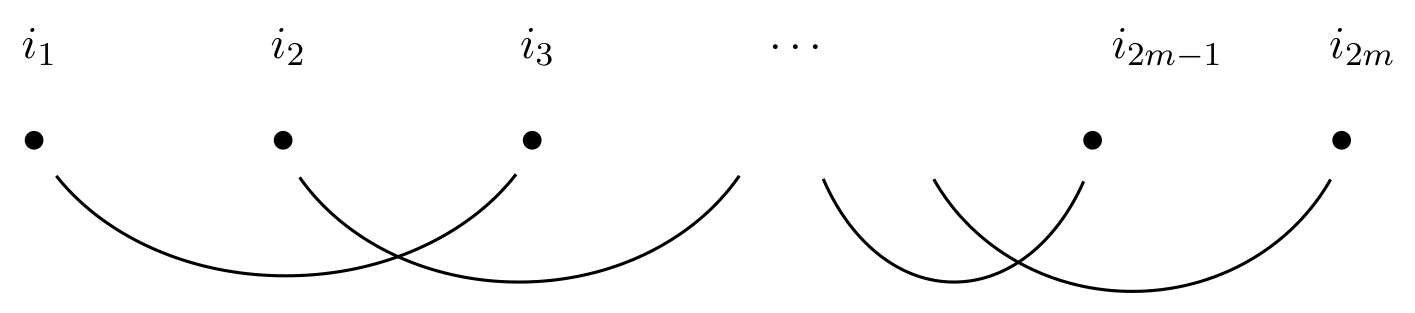
\includegraphics[width=0.92\textwidth]{figures/fig_p141_b.png}
\end{center}
% [图：原书 p.140]

% [原文 p.141]
对于连接 $i$ 与 $j$ 的每条边，给它配上因子 $\hs(Q^{-1})^{ij}$。

\begin{example}{2.8.1}
  \textbf{（两点函数）}两点函数
  \[
  \langle x^ix^j\rangle_x=\hs(Q^{-1})^{ij}
  \]
  由 $Q$ 的逆矩阵给出。$(Q^{-1})^{ij}$ 也称为“传播子”。
  \begin{center}
  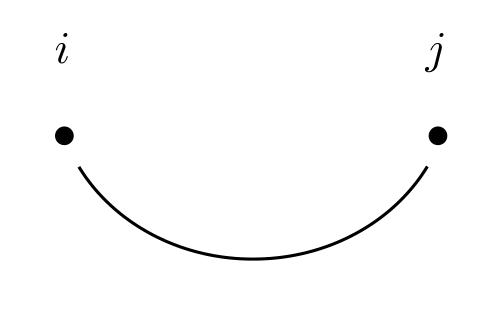
\includegraphics[width=0.22\textwidth]{figures/fig_p142_a.png}
  \end{center}
  % [图：原书 p.141]
\end{example}

\begin{example}{2.8.2}
  如下四点函数由下式算出
  \[
  \langle x^ix^jx^kx^l\rangle_x
  =\wickfour{0/1,2/3}+\wickfour{0/2,1/3}+\wickfour{0/3,1/2}
  \]
  \[
  =\hs^2\Bigl[(Q^{-1})^{ij}(Q^{-1})^{kl}
  +(Q^{-1})^{ik}(Q^{-1})^{jl}+(Q^{-1})^{il}(Q^{-1})^{jk}\Bigr].
  \]
\end{example}

我们也可以考虑平移 $x\to x+a$，以此加入“背景”：
\[
\langle f(x+a)\rangle_x=\int_{\R^n}\Omega f(x+a),
\]
它现在是 $a$ 的函数。类似的论证给出
\[
\langle f(x+a)\rangle_x=\ee^{\frac{\hs}{2}Q^{-1}(\frac{\pa}{\pa a})}f(a).
\]
若 $f(x)=x^{i_1}x^{i_2}\cdots x^{i_k}$，则此时的 威克定理是对部分配对的求和
\begin{center}
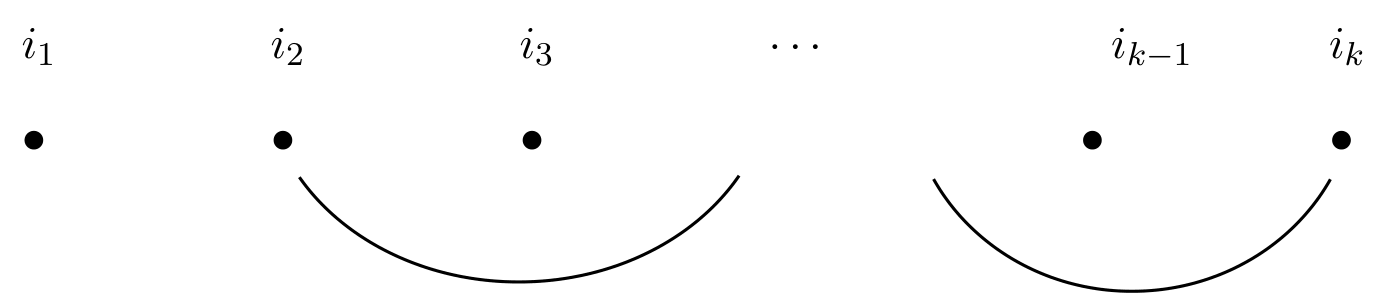
\includegraphics[width=0.75\textwidth]{figures/fig_p142_b.png}
\end{center}
% [图：原书 p.141]
我们把传播子配给已配对的指标，把 $a^i$ 配给未配对的指标 $i$。

\begin{example}{2.8.3}
  设 $f(x)=x^ix^jx^kx^l$。则
  \[
  \begin{gathered}
  \langle f(x+a)\rangle_x
  =\wickfour{}+\wickfour{0/1}+\wickfour{0/2}+\wickfour{0/3}\\
  +\wickfour{1/2}+\wickfour{1/3}+\wickfour{2/3}\\
  +\wickfour{0/1,2/3}+\wickfour{0/2,1/3}+\wickfour{0/3,1/2}
  \end{gathered}
  \]
  \[
  \begin{aligned}
  &=a^ia^ja^ka^l+\hs\Bigl[(Q^{-1})^{ij}a^ka^l+(Q^{-1})^{ik}a^ja^l
  +(Q^{-1})^{il}a^ja^k\\
  &\qquad\qquad +(Q^{-1})^{jk}a^ia^l+(Q^{-1})^{jl}a^ia^k
  +(Q^{-1})^{kl}a^ia^j\Bigr]\\
  &\quad+\hs^2\Bigl[(Q^{-1})^{ij}(Q^{-1})^{kl}
  +(Q^{-1})^{ik}(Q^{-1})^{jl}+(Q^{-1})^{il}(Q^{-1})^{jk}\Bigr].
  \end{aligned}
  \]
\end{example}

% [原文 p.142]
\subsection{费曼图展开}

现在考虑如下形式的积分
\[
\sqrt{\det Q}\int_{\R^n}\prod_{i=1}^n\frac{\rd x^i}{\sqrt{2\pi\hs}}\,
\ee^{-\frac1\hs S(x)},
\]
其中
\[
S(x)=\frac12Q(x)-\frac{\lambda}{3!}I(x).
\]
这里 $Q(x)=\sum_{i,j}Q_{ij}x^ix^j$ 与前面一样是正定二次型，而
\[
I(x)=\sum_{i,j,k}I_{ijk}x^ix^jx^k
\]
是三次多项式，称为“\emph{相互作用}”（interaction）。常数 $I_{ijk}$ 参数化这些三次多项式，常数 $\lambda$ 称为“\emph{耦合常数}”（coupling constant）。

由于三次项在两端都趋于 $\pm\infty$，且增长快于二次项，上述积分干脆就是“发散的”。要让它有意义，本质上只有两条出路：

① 把 $x^i$ 复化为复变量 $z^i$，并把积分围道
\[
\R^n\subset\C^n\qquad\Longrightarrow\qquad\Gamma\subset\C^n
\]
换成另一条围道 $\Gamma$，使积分收敛。“艾里积分”就是这样的例子。这一方法通常称为非微扰方法。

② 把 $\lambda$ 当作微扰参数，计算渐近级数。这一方法通常称为微扰方法。

这里我们聚焦微扰方法 ②。让我们把
\[
\Bigl(\sqrt{\det Q}\int_{\R^n}\prod_{i=1}^n\frac{\rd x^i}{\sqrt{2\pi\hs}}
\,\ee^{-\frac1\hs S(x)}\Bigr)
=\Bigl(\int_{\R^n}\Omega\,\ee^{\frac{\lambda}{3!\hs}I(x)}\Bigr)
=\Bigl\langle \ee^{\frac{\lambda}{3!\hs}I(x)}\Bigr\rangle_x
\]
改写。这里 $\Omega=\sqrt{\det Q}\prod_{i=1}^n\frac{\rd x^i}{\sqrt{2\pi\hs}}
\ee^{-\frac1{2\hs}Q(x)}$ 是前面的概率密度。现在把这个发散积分重定义为幂级数
\[
\sum_{m=0}^\infty\frac{\lambda^m}{m!\hs^m}
\Bigl\langle\Bigl(\frac1{3!}I(x)\Bigr)^m\Bigr\rangle_x.
\]
这里的每一项 $\bigl\langle\bigl(\frac1{3!}I(x)\bigr)^m\bigr\rangle_x$ 都有确定的值，可用 威克定理算出。由此将得到这一幂级数的组合图公式。

\begin{definition}{2.8.4}
  所谓一个\emph{图}（graph）$\Gamma$，是指如下数据
  \begin{itemize}
  \item $V(\Gamma)=$ 顶点集；
  \item $HE(\Gamma)=$ 半边集；
  \tutornote{原文此处在 $\gamma$ 与 $\Gamma$ 之间混用，译文统一记为 $\Gamma$。}
  % [原文 p.143]（原书在此条处翻页）
  \item $i_\Gamma:HE(\Gamma)\to V(\Gamma)$ 关联映射；
  \item $E(\Gamma)$：$HE(\Gamma)$ 上的完美匹配，即把半边分成两两一组的集合。每一对称为一条“\emph{边}”（edge）；
  \item 对每个 $v\in V(\Gamma)$，$\#\{i_\Gamma^{-1}(v)\}$ 称为 $v$ 的\emph{度数}（valency）。
  \end{itemize}
\end{definition}

\begin{example}{2.8.5}
  考虑如下 $\Theta$ 图
  \begin{center}
  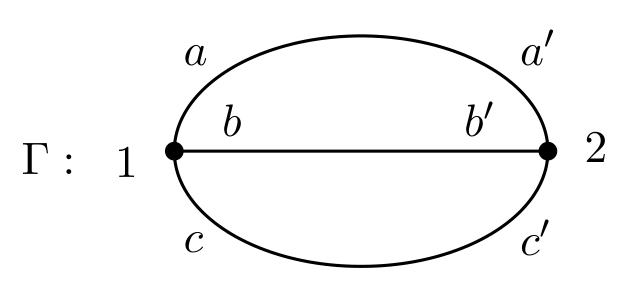
\includegraphics[width=0.34\textwidth]{figures/fig_p144_a.png}
  \end{center}
  % [图：原书 p.143]
  这里 $V=\{1,2\}$，$HE=\{a,b,c,a',b',c'\}$，$E=\{(a,a'),(b,b'),(c,c')\}$。关联映射为
  \[
  \begin{array}{rcl}
  i_\Gamma:HE&\longrightarrow&V\\
  \{a,b,c\}&\longmapsto&1\\
  \{a',b',c'\}&\longmapsto&2
  \end{array}
  \]
  顶点 1 与 2 的度数都是 3。
\end{example}

\begin{definition}{2.8.6}
  图 $\Gamma$ 与 $\Gamma'$ 之间的一个\emph{图同构}（graph isomorphism）是一对双射
  \[
  \sigma_V:V(\Gamma)\longrightarrow V(\Gamma'),\qquad
  \sigma_{HE}:HE(\Gamma)\longrightarrow HE(\Gamma'),
  \]
  它们与关联映射相容（即下图交换）
  \[
  \begin{array}{ccc}
  HE(\Gamma)&\xrightarrow{\ \sigma_{HE}\ }&HE(\Gamma')\\[1mm]
  \big\downarrow{\scriptstyle i_\Gamma}&&\big\downarrow{\scriptstyle i'_{\Gamma'}}\\[1mm]
  V(\Gamma)&\xrightarrow{\ \sigma_V\ }&V(\Gamma')
  \end{array}
  \]
  并与边相容：对任意 $a,b\in HE(\Gamma)$，
  \[
  (a,b)\in E(\Gamma)\quad\Longleftrightarrow\quad
  (\sigma_{HE}(a),\sigma_{HE}(b))\in E(\Gamma').
  \]
  $\Gamma$ 的一个\emph{自同构}（automorphism）是同构 $\sigma:\Gamma\to\Gamma$。记
  \[
  \Aut(\Gamma)=\Gamma\text{ 的自同构群}.
  \]
\end{definition}

\begin{example}{2.8.7}
  考虑
  \begin{center}
  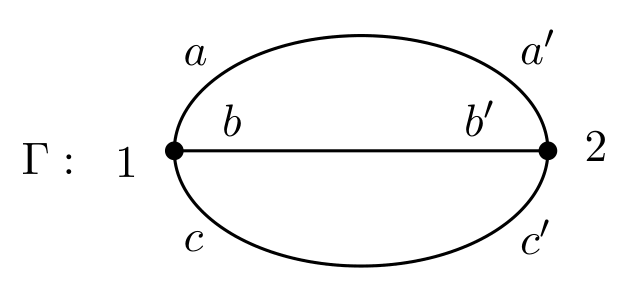
\includegraphics[width=0.34\textwidth]{figures/fig_p144_b.png}
  \end{center}
  % [图：原书 p.143]
  这里 $HE=\{a,b,c,a',b',c'\}$，$V=\{1,2\}$，$E=\{(a,a'),(b,b'),(c,c')\}$，关联映射同上。下面是 $\Gamma$ 的两个自同构的例子
\end{example}

% [原文 p.144]
①
\[
\begin{aligned}
&\sigma_V:(1,2)\longrightarrow(2,1),\\
&\sigma_{HE}:(a,b,c,a',b',c')\longrightarrow(a',b',c',a,b,c);
\end{aligned}
\]
②
\[
\begin{aligned}
&\sigma_V:(1,2)\longrightarrow(1,2),\\
&\sigma_{HE}:(a,b,c,a',b',c')\longrightarrow(b,c,a,b',c',a').
\end{aligned}
\]
类似地可得 $\Aut(\Gamma)=\Z_2\times S_3$。这里 $\Z_2$ 对应两个顶点的置换，$S_3$ 对应三条边的置换。

\begin{example}{2.8.8}
  考虑
  \begin{center}
  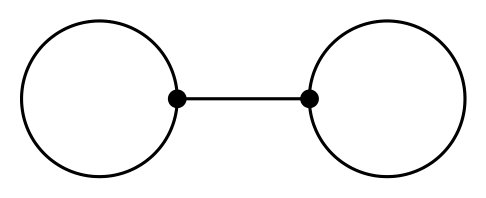
\includegraphics[width=0.26\textwidth]{figures/fig_p145_a.png}
  \end{center}
  % [图：原书 p.144]
  可得 $\Aut(\Gamma)=\Z_2\times\Z_2\times\Z_2$。
\end{example}

现在考虑
\[
\langle I(x)^m\rangle_x
=\bigl\langle\underbrace{I(x)I(x)\cdots I(x)}_{m}\bigr\rangle_x
\]
的计算。每个 $I(x)$ 给出一个有 3 条半边的顶点
\begin{center}
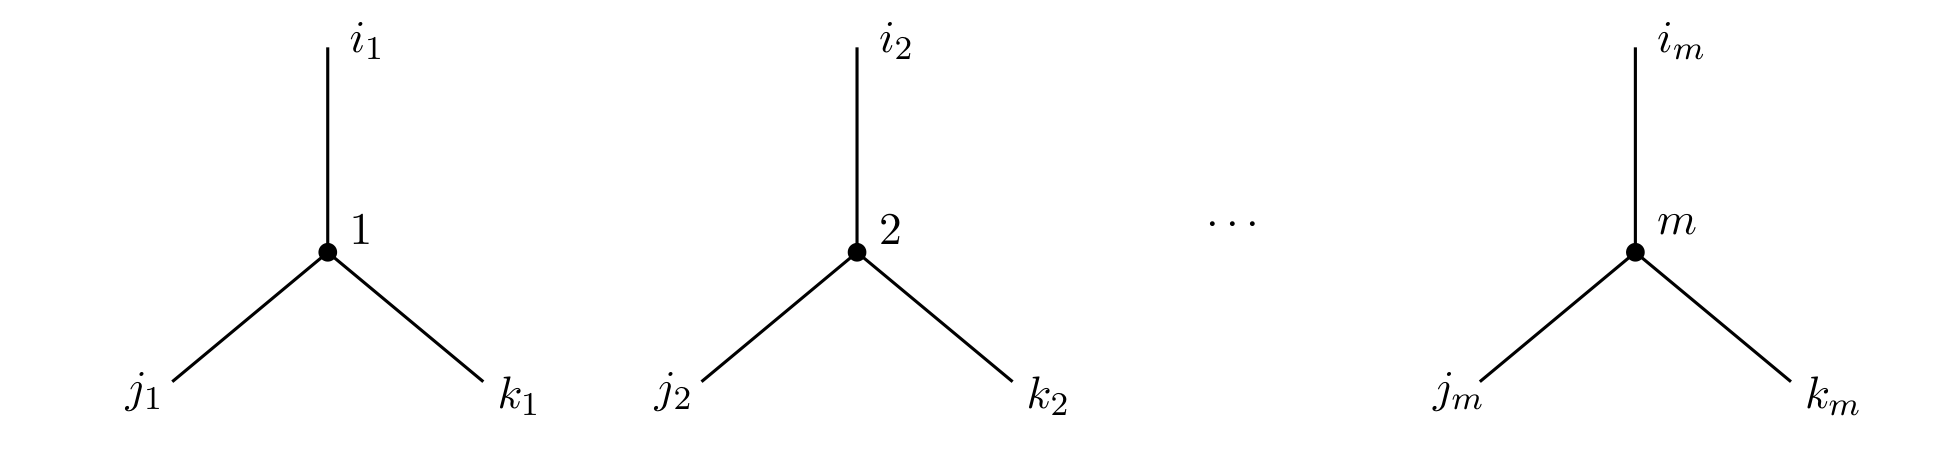
\includegraphics[width=0.86\textwidth]{figures/fig_p145_v.png}
\end{center}
% [图：原书 p.144]
\[
\begin{aligned}
\text{顶点集}&\qquad V=\{1,2,\cdots,m\}\\
\text{半边集}&\qquad HE=\{i_1,j_1,k_1,i_2,j_2,k_2,\cdots,i_m,j_m,k_m\}\\
\text{关联映射}&\qquad i:\{i_s,j_s,k_s\}\longrightarrow\{s\}
\end{aligned}
\]
由 威克定理，$\langle I(x)^m\rangle_x$ 是对完美匹配 $E$ 的求和
\[
\langle I(x)^m\rangle_x=\sum_{E\in Y}\hs^{|E(\Gamma_E)|}\omega_{\Gamma_E}.
\]
这里 $Y=\{HE\text{ 的完美匹配}\}$，而 $\Gamma_E$ 是把配对 $E$ 赋给顶点集 $V$ 与半边集 $HE$ 所得的图。

对每个图 $\Gamma$，$\omega_\Gamma$ 是按如下方式赋值得出的数
\begin{center}
\begin{tabular}{lll}
① 每个顶点 & $\trivertex$ & $\Longrightarrow\ I_{ijk}$；\\[2mm]
② 每条边 & $\edgeij$ & $\Longrightarrow\ (Q^{-1})^{ij}$；
\end{tabular}
\end{center}

% [原文 p.145]
③ 对指标求和。

\begin{example}{2.8.9}
  考虑
  \begin{center}
  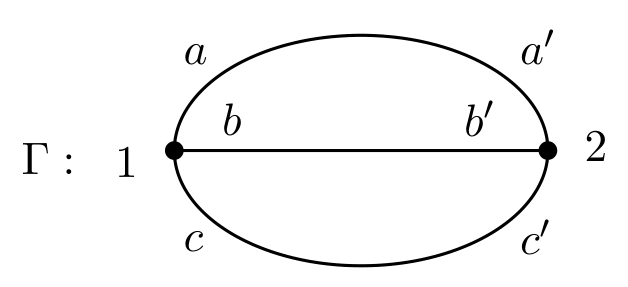
\includegraphics[width=0.34\textwidth]{figures/fig_p146_a.png}
  \end{center}
  % [图：原书 p.145]
  \[
  \omega_\Gamma=\sum_{\substack{i_1,j_1,k_1\\i_2,j_2,k_2}}
  I_{i_1j_1k_1}I_{i_2j_2k_2}(Q^{-1})^{i_1i_2}(Q^{-1})^{j_1j_2}(Q^{-1})^{k_1k_2}.
  \]
\end{example}
显然，若 $\Gamma$ 与 $\Gamma'$ 同构，则 $\omega_\Gamma=\omega_{\Gamma'}$。

这里所有图都是三价的（每个顶点度数为 3）。保持关联映射的双射
\[
\sigma_V:V\longrightarrow V,\qquad \sigma_{HE}:HE\longrightarrow HE
\]
之集为
\[
G=\underbrace{S_m}_{\text{置换顶点}}\times
\underbrace{(S_3)^m}_{\text{置换半边}}.
\]
我们有自然的 $G$-作用在 $Y$ 上，其轨道为
\[
Y/G=\{m\text{ 个顶点的三价图的同构类}\}.
\]
于是
\begin{align*}
\frac{1}{m!(3!)^m}\langle I(x)^m\rangle_x
&=\frac{1}{|G|}\sum_{\Gamma\in Y/G}\frac{|G|}{|\Aut(\Gamma)|}
\omega_\Gamma\hs^{|E(\Gamma)|}\\
&=\sum_{\substack{\Gamma:\ \text{三价图}\\\text{有 }m\text{ 个顶点}}}
\frac{\omega_\Gamma}{|\Aut(\Gamma)|}\hs^{|E(\Gamma)|}.
\end{align*}
我们也可以按同构把不连通图归并，进一步细化这一公式。这引出了如下费曼图展开公式（细节留给读者）。

\begin{proposition}{2.8.10}（费曼图展开公式）
  对渐近幂级数，有如下组合图展开公式
  \begin{align*}
  \Bigl\langle\ee^{\frac{\lambda}{3!\hs}I(x)}\Bigr\rangle_x
  &:=\sum_{m=0}^\infty\frac{\lambda^m}{m!\hs^m}
  \Bigl\langle\Bigl(\frac1{3!}I(x)\Bigr)^m\Bigr\rangle_x\\
  &=\sum_{\Gamma:\ \text{三价}}\hs^{|E(\Gamma)|-|V(\Gamma)|}
  \lambda^{|V(\Gamma)|}\frac{\omega_\Gamma}{|\Aut(\Gamma)|}\\
  &=\exp\Biggl(\sum_{\substack{\Gamma:\ \text{连通}\\\text{三价}}}
  \lambda^{|V(\Gamma)|}\hs^{l(\Gamma)-1}
  \frac{\omega_\Gamma}{|\Aut(\Gamma)|}\Biggr).
  \end{align*}
\end{proposition}

% [原文 p.146]
这里对连通图 $\Gamma$，
\[
l(\Gamma)=|E(\Gamma)|-|V(\Gamma)|+1=1-\chi(\Gamma)
\]
称为 $\Gamma$ 的\emph{圈数}（loop number）。
\begin{center}
\begin{tabular}{cc}
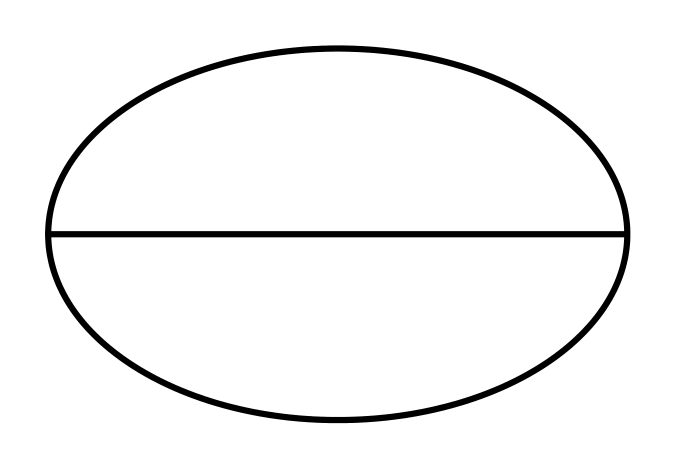
\includegraphics[width=0.25\textwidth]{figures/fig_p147_b.png} &
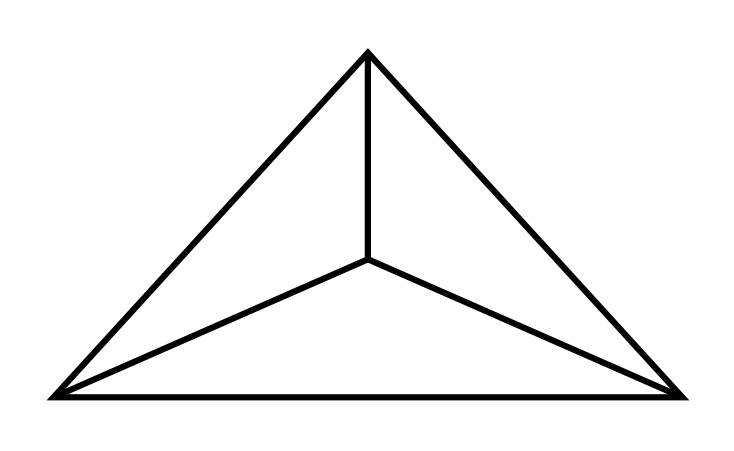
\includegraphics[width=0.23\textwidth]{figures/fig_p147_a.png}\\[1mm]
$l(\Gamma)=3-2+1=2$ & $l(\Gamma)=6-4+1=3$
\end{tabular}
\end{center}
% [图：原书 p.146]

一般而言，若相互作用包含所有可能次数的项
\[
\frac{\lambda_3}{3!}I_3(x)+\frac{\lambda_4}{4!}I_4(x)+\cdots
+\frac{\lambda_m}{m!}I_m(x)+\cdots,
\]
则级数展开将包含所有可能的图，其中度数为 $m$ 的每个顶点类似地配上 $I_m$。一般的费曼图展开公式为
\[
\Bigl\langle \ee^{\frac1\hs\bigl(\sum_{m\ge3}\frac{\lambda_m}{m!}I_m(x)\bigr)}
\Bigr\rangle_x
\overset{\text{渐近}}{\simeq}
\exp\Biggl(\sum_{\substack{\Gamma:\ \text{连通}\\\text{图}}}
\Bigl(\prod_{m\ge3}\lambda_m^{|V_m(\Gamma)|}\Bigr)
\hs^{l(\Gamma)-1}\frac{\omega_\Gamma}{|\Aut(\Gamma)|}\Biggr),
\]
其中 $V_m(\Gamma)$ 是度数为 $m$ 的顶点之集。

\subsection{再论外尔量子化}

下面把费曼图的组合公式用到量子力学情形。相关的空间由相空间上以时间为参数的路径组成。为简单起见，取相空间为 $\R^2$；讨论容易推广到 $\R^{2n}$。

用 $\gamma(t)=(\mathbb X(t),\mathbb P(t))$ 表示粒子在相空间 $\R^2$ 上的轨道。于是 $\gamma$ 可看作一个映射
\[
\gamma:\R\longrightarrow\R^2,\qquad t\longmapsto(\mathbb X(t),\mathbb P(t)).
\]
记
\[
\mathcal E=\operatorname{Map}(\R,\R^2).
\]
作用量 $S$ 可看作 $\mathcal E$ 上的函数（其定义域适当即可，与当前讨论无关）
\[
S:\mathcal E\longrightarrow\R,\qquad
S[\gamma]=\int\bigl(\mathbb P\dot{\mathbb X}-\mathcal H\bigr)\rd t.
\]
我们关心如下期望值
\[
\langle\mathcal O\rangle_\gamma
=\frac{\int_{\mathcal E}[D\gamma]\,\ee^{\frac{\ii}{\hs}S[\gamma]}\mathcal O[\gamma]}
{\int_{\mathcal E}[D\gamma]\,\ee^{\frac{\ii}{\hs}S[\gamma]}},
\]
% [原文 p.147]
其中 $\mathcal O$ 是 $\mathcal E$ 上适当的函数，称为\emph{可观测量}（observable）。

先看不含哈密顿量 $\mathcal H$ 的自由情形，即
\[
S[\gamma]=S_0[\gamma]=\int\mathbb P\dot{\mathbb X}\,\rd t.
\]

后文会看到，零哈密顿量情形具有拓扑本性。

上述积分在无穷维路径空间 $\mathcal E$ 上进行，本来就没有良好定义。第 2 章把路径积分当作有限维近似的极限。时间为虚时，它与维纳测度积分有关。

本节改用另一种微扰方法：可以借用有限维的结果，把平行的组合公式搬到无穷维情形。下面看它在实践中如何运作。

先比较有限维与无穷维两种情形。
\begin{center}
\small
\begin{tabular}{@{}l@{\hspace{5pt}}l@{\hspace{5pt}}l@{}}
\toprule
 & 有限维 & 无穷维\\ \midrule
空间 & $\R^n$ & $\mathcal E=\operatorname{Map}(\R,\R^2)$\\
变量 & $x^i$ & $\gamma(t)$\\
指标 & $i\in\{1,2,\cdots,n\}$ & $t\in\R$\\
求和 & $\sum_i$ & $\int_\R\rd t$\\
作用量 & $Q(x)=\sum_{i,j}Q_{ij}x^ix^j$ & $S_0[\gamma]=\int\mathbb P\dot{\mathbb X}\,\rd t$\\
密度 & $\ee^{-\frac{1}{2\hs}Q(x)}$ & $\ee^{\frac{\ii}{\hs}S_0[\gamma]}$\\
\bottomrule
\end{tabular}
\end{center}

有限维情形中，两点函数
\[
\langle x^ix^j\rangle_x=\hs(Q^{-1})^{ij}
\]
作为计算一般期望值的基本构件起核心作用。它称为“\emph{传播子}”（propagator），由二次配对 $Q$ 的逆矩阵给出。

无穷维情形看起来完全一样。自由作用量
\[
S_0[\gamma]=\int\mathbb P\dot{\mathbb X}\,\rd t
\]
关于 $\gamma=(\mathbb X,\mathbb P)$ 是二次的。写（暂且忽略边界行为）
\[
\begin{aligned}
S_0[\gamma]&=\frac12\int\bigl(\mathbb P\dot{\mathbb X}-\mathbb X\dot{\mathbb P}\bigr)\rd t\\
&=\frac12\int
\begin{bmatrix}\mathbb X&\mathbb P\end{bmatrix}
\begin{bmatrix}0&-\dfrac{\rd}{\rd t}\\[2mm] \dfrac{\rd}{\rd t}&0\end{bmatrix}
\begin{bmatrix}\mathbb X\\ \mathbb P\end{bmatrix}\rd t.
\end{aligned}
\]
\tutornote{原文此式矩阵只印出两个 $-\rd/\rd t$、$\rd/\rd t$ 块，两个零块从略；译文按 2×2 矩阵补全。}
于是
\[
\ee^{\frac{\ii}{\hs}S_0[\gamma]}
=\exp\Bigl(-\frac{1}{2\hs}\Bigl(\frac1{\ii}\int
\begin{bmatrix}\mathbb X(t)&\mathbb P(t)\end{bmatrix}
\begin{bmatrix}0&-\dfrac{\rd}{\rd t}\\[2mm] \dfrac{\rd}{\rd t}&0\end{bmatrix}
\begin{bmatrix}\mathbb X(t)\\ \mathbb P(t)\end{bmatrix}\rd t\Bigr)\Bigr).
\]
与有限维情形
\[
\ee^{-\frac{1}{2\hs}\sum_{i,j}Q_{ij}x^ix^j}
\]
% [原文 p.148]
比较可知，逆矩阵 $Q^{-1}$ 的类比物是
\[
\ii\begin{bmatrix}0&-\dfrac{\rd}{\rd t}\\[2mm] \dfrac{\rd}{\rd t}&0\end{bmatrix}^{-1}.
\]

分析中，微分算子的逆通常用积分核表示，称为\emph{格林函数}（Green's function）。$\dfrac{\rd}{\rd t}$ 的格林函数是满足
\[
\frac{\pa}{\pa t_1}G(t_1,t_2)=\delta(t_1-t_2)
\]
的函数 $G(t_1,t_2)$。这里 $\delta(t_1-t_2)$ 可看作 $\delta_{ij}$ 的无穷维类比。

用 $G(t_1,t_2)$ 可以写出
\[
\begin{bmatrix}0&-\dfrac{\pa}{\pa t_1}\\[2mm] \dfrac{\pa}{\pa t_1}&0\end{bmatrix}
\begin{bmatrix}0&G(t_1,t_2)\\ -G(t_1,t_2)&0\end{bmatrix}
=\begin{bmatrix}\delta(t_1-t_2)&0\\ 0&\delta(t_1-t_2)\end{bmatrix}.
\]
右端可看作无穷维单位矩阵的 $(t_1,t_2)$ 元素。于是上述逆矩阵的 $(t_1,t_2)$ 元素可写成
\[
\ii\begin{bmatrix}0&-\dfrac{\rd}{\rd t}\\[2mm] \dfrac{\rd}{\rd t}&0\end{bmatrix}^{-1}_{t_1,t_2}
=\begin{bmatrix}0&\ii G(t_1,t_2)\\ -\ii G(t_1,t_2)&0\end{bmatrix}.
\]
据此可用这个逆“定义”两点函数
\[
\begin{cases}
\langle\mathbb X(t_1)\mathbb P(t_2)\rangle_\gamma:=\ii\hs G(t_1,t_2),\\[1mm]
\langle\mathbb P(t_1)\mathbb X(t_2)\rangle_\gamma:=-\ii\hs G(t_1,t_2),\\[1mm]
\langle\mathbb X(t_1)\mathbb X(t_2)\rangle_\gamma
=\langle\mathbb P(t_1)\mathbb P(t_2)\rangle_\gamma=0.
\end{cases}
\]
剩下要解 $G(t_1,t_2)$。上式要求 $G$ 满足
\[
G(t_1,t_2)=-G(t_2,t_1).
\]
$\dfrac{\rd}{\rd t}$ 的这种格林函数由下式显式给出
\[
G(t_1,t_2)=\frac12\sgn(t_1-t_2)
=\begin{cases}
\dfrac12&t_1>t_2,\\[2mm]
0&t_1=t_2,\\[2mm]
-\dfrac12&t_1<t_2.
\end{cases}
\]
\begin{center}
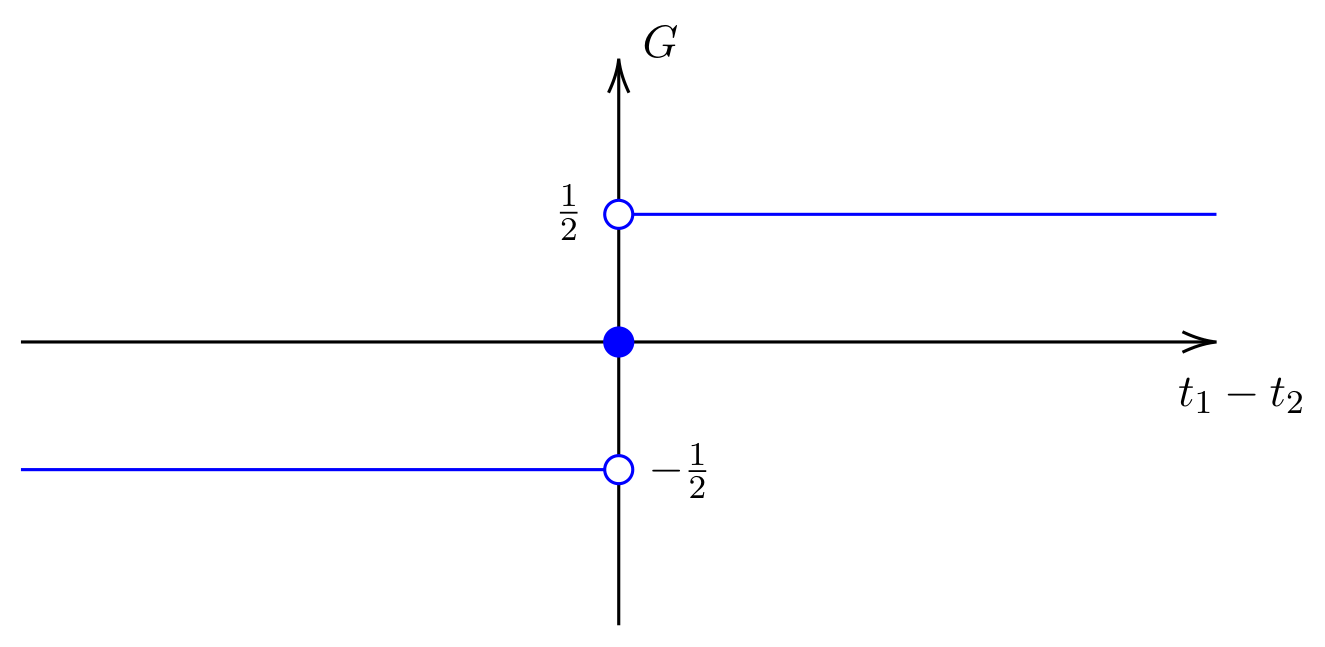
\includegraphics[width=0.42\textwidth]{figures/fig_p149_a.png}
\end{center}
% [图：原书 p.148]

% [原文 p.149]
事实上，对任意紧支检验函数 $f(t)$，
\[
\begin{aligned}
-\int_\R\rd t_1\,G(t_1,t_2)f'(t_1)
&=\frac12\int_{-\infty}^{t_2}\rd t_1\,f'(t_1)
-\frac12\int_{t_2}^{\infty}\rd t_1\,f'(t_1)\\
&=\frac12f(t_2)-\frac12\bigl(-f(t_2)\bigr)=f(t_2).
\end{aligned}
\]
故
\[
\frac{\pa}{\pa t_1}G(t_1,t_2)=\delta(t_1-t_2)
\]
作为分布等式成立。

总结起来，我们关心如下两点函数
\[
\langle\mathbb X(t_1)\mathbb P(t_2)\rangle_\gamma\ \text{“}=\text{”}\
\frac{\int[D\gamma]\,\ee^{\frac{\ii}{\hs}S_0[\gamma]}\mathbb X(t_1)\mathbb P(t_2)}
{\int[D\gamma]\,\ee^{\frac{\ii}{\hs}S_0[\gamma]}}.
\]
虽然事先并不知道路径积分测度的精确信息，对照有限维高斯积分仍可得到合理结果
\[
\langle\mathbb X(t_1)\mathbb P(t_2)\rangle_\gamma
:=\ii\hs G(t_1,t_2)=\frac{\ii\hs}{2}\sgn(t_1-t_2).
\]
下文就用这一公式定义两点函数。

注意这个两点函数（即传播子）并不依赖 $t_1,t_2$ 的具体取值，只依赖它们的相对位置
\[
\langle\mathbb X(t_1)\mathbb P(t_2)\rangle_\gamma
=\begin{cases}
\dfrac{\ii\hs}{2}&t_1>t_2,\\[2mm]
0&t_1=t_2,\\[2mm]
-\dfrac{\ii\hs}{2}&t_1<t_2.
\end{cases}
\]
这显示该模型的拓扑本性；事实也确实如此。

现在设 $f(x,p)$ 与 $g(x,p)$ 是两个多项式。把它们画在时间轴上
\begin{center}
\timeline{1.0/{$t_1$}/{$g$},3.0/{$t_2$}/{$f$}}
\end{center}
% [图：原书 p.149，本图按原文重绘，图内标注已译为中文；原图无题注]
再由如下关联定义相空间上的一个新函数
\[
\bigl\langle f(x+\mathbb X(t_2),p+\mathbb P(t_2))\,
g(x+\mathbb X(t_1),p+\mathbb P(t_1))\bigr\rangle_\gamma.
\]
这里在时刻 $t_1$ 用 $g$、在时刻 $t_2$ 用 $f$，让量子涨落 $\mathbb X(t),\mathbb P(t)$ 扰动变量 $x,p$。等价地，可把 $x,p$ 看作“背景”平移。该关联函数依赖背景变量 $\{x,p\}$，给出相空间上的一个函数。

用 威克定理计算这一关联。把 $f$ 与 $g$ 各表示成一个顶点，其度数等于多项式次数
\begin{center}
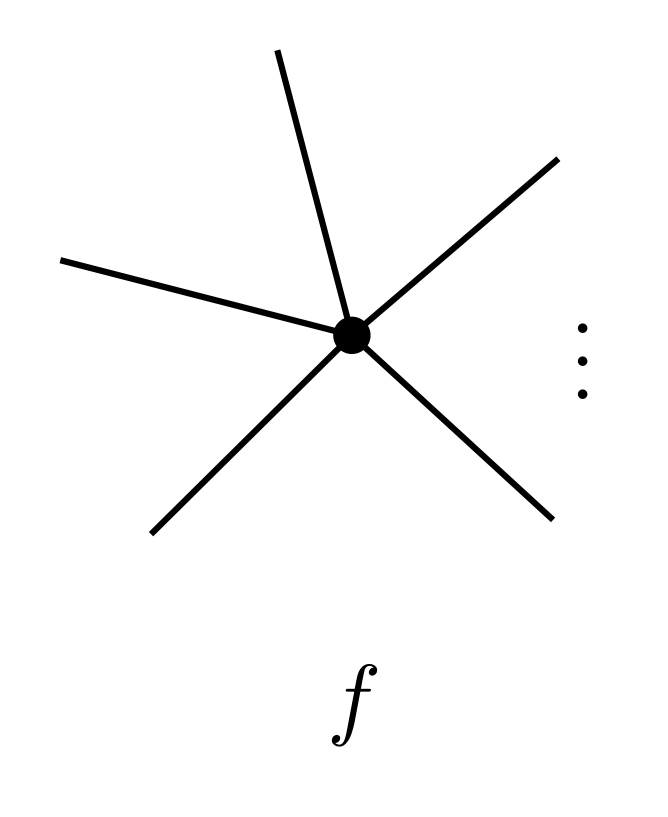
\includegraphics[width=0.14\textwidth]{figures/fig_p150_a.png}\hspace{14mm}
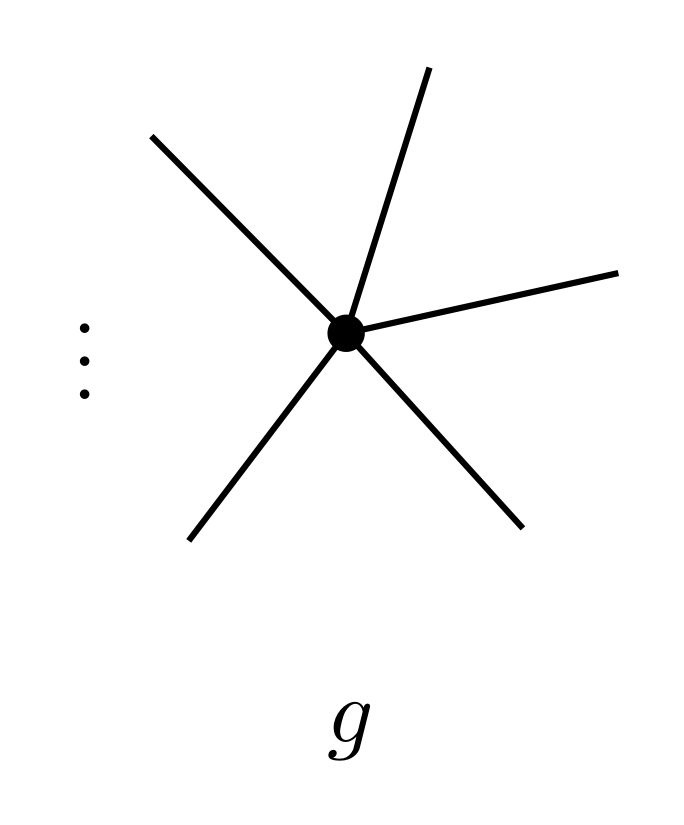
\includegraphics[width=0.14\textwidth]{figures/fig_p150_b.png}
\end{center}
% [图：原书 p.149]

% [原文 p.150]
威克定理说
\begin{center}

\includegraphics[width=0.88\textwidth]{figures/fig_p151_a.png}
\end{center}
% [图：原书 p.150]
这里每条未配对的半边按原顶点配上 $x$ 或 $p$。至于配对的半边
\begin{center}
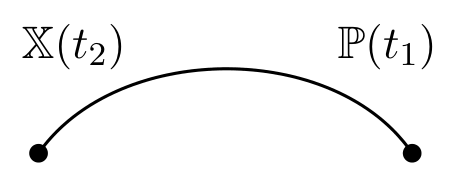
\includegraphics[width=0.20\textwidth]{figures/fig_p151_b.png}
\quad$\Longrightarrow$\quad
$\langle\mathbb X(t_2)\mathbb P(t_1)\rangle_\gamma=\dfrac{\ii}{2}\hs$；\\[3mm]
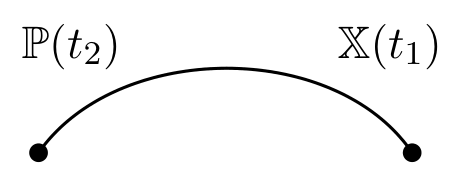
\includegraphics[width=0.20\textwidth]{figures/fig_p151_c.png}
\quad$\Longrightarrow$\quad
$\langle\mathbb P(t_2)\mathbb X(t_1)\rangle_\gamma=-\dfrac{\ii}{2}\hs$。
\end{center}
% [图：原书 p.150]
有 $m$ 个传播子的图会因置换各条边而带有自同构群 $S_m$，在费曼图展开中贡献 $\dfrac1{m!}$。于是
\[
\begin{aligned}
&\bigl\langle f(x+\mathbb X(t_2),p+\mathbb P(t_2))\,
g(x+\mathbb X(t_1),p+\mathbb P(t_1))\bigr\rangle_\gamma\\
&\quad=f(x,p)\,
\ee^{\frac{\ii}{2}\hs\bigl(
\overleftarrow{\dfrac{\pa}{\pa x}}\overrightarrow{\dfrac{\pa}{\pa p}}
-\overleftarrow{\dfrac{\pa}{\pa p}}\overrightarrow{\dfrac{\pa}{\pa x}}\bigr)}
g(x,p)=(f*_{\hs}g)(x,p),
\end{aligned}
\]
这正是 Moyal 乘积。

可以把时间轴
\begin{center}
\timeline{1.0/{$t_1$}/{$g$},3.0/{$t_2$}/{$f$}}
\end{center}
% [图：原书 p.150，本图按原文重绘，图内标注已译为中文；原图无题注]
想成：在时刻 $t_1$ 插入算子 $g$，然后在较晚的时刻 $t_2$ 插入算子 $f$。总效果是两算子的复合，量子力学中由 Moyal 乘积 $f*_{\hs}g$ 表示。

这一图景也给 Moyal 乘积 $*_{\hs}$ 的结合性一个简单解释。给定三个函数 $f,g,h$，按时间顺序插入
\begin{center}
\timeline{0.8/{$t_1$}/{$h$},2.6/{$t_2$}/{$g$},4.4/{$t_3$}/{$f$}}
\end{center}
% [图：原书 p.150，本图按原文重绘，图内标注已译为中文；原图无题注]
考虑关联
\[
\bigl\langle f(x+\mathbb X(t_3),p+\mathbb P(t_3))\,
g(x+\mathbb X(t_2),p+\mathbb P(t_2))\,
h(x+\mathbb X(t_1),p+\mathbb P(t_1))\bigr\rangle_\gamma.
\]

% [原文 p.151]
这一值在时间位置的局部形变下不变，只与插入的顺序有关。由前面的计算
\[
\begin{aligned}
(f*_{\hs}g)*_{\hs}h
&=\lim_{t_1\to t_2^-}\lim_{t_3\to t_2^+}
\bigl\langle f(x+\mathbb X(t_3),p+\mathbb P(t_3))\\
&\qquad\times g(x+\mathbb X(t_2),p+\mathbb P(t_2))\,
h(x+\mathbb X(t_1),p+\mathbb P(t_1))\bigr\rangle_\gamma,\\[1mm]
f*_{\hs}(g*_{\hs}h)
&=\lim_{t_3\to t_2^+}\lim_{t_1\to t_2^-}
\bigl\langle f(x+\mathbb X(t_3),p+\mathbb P(t_3))\\
&\qquad\times g(x+\mathbb X(t_2),p+\mathbb P(t_2))\,
h(x+\mathbb X(t_1),p+\mathbb P(t_1))\bigr\rangle_\gamma.
\end{aligned}
\]
上述关联的拓扑本性意味着
\[
(f*_{\hs}g)*_{\hs}h=f*_{\hs}(g*_{\hs}h).
\]

\subsection{$S^1$ 关联}

下面引入拓扑，把量子力学模型放到 $S^1$ 上
\[
\gamma(\theta)=\bigl(\mathbb X^i(\theta),\mathbb P_i(\theta)\bigr):
S^1\longrightarrow\R^{2n}.
\]
这里 $\theta\in S^1$ 是角变量，并认同
\[
\theta\sim\theta+1.
\]
\begin{center}
\begin{tikzpicture}[baseline=0pt,x=0.55cm,y=0.55cm]
  \draw (0,0) circle (0.9);
  \node[below,inner sep=2pt,font=\small] at (0,-1.05) {$S^1$};
  \node[above,inner sep=4pt,font=\small] at (2.6,0.28) {$\theta\sim\theta+1$};
  \draw[-{Latex[length=2mm]}] (1.5,0)--(3.4,0)
    node[midway,above,inner sep=2pt,font=\small] {$\gamma$};
  \node[right,inner sep=3pt,font=\small] at (3.55,0) {$\R^{2n}$};
\end{tikzpicture}
\end{center}
% [图：原书 p.151，本图按原文重绘，图内标注已译为中文；原图无题注]

\subsubsection*{$S^1$ 传播子}

与前面一样考虑自由作用量
\[
S_0[\gamma]=\int_{S^1}\mathbb P_i(\theta)\dot{\mathbb X}^i(\theta)\,\rd\theta,
\qquad
\dot{\mathbb X}^i(\theta)=\frac{\rd\mathbb X^i}{\rd\theta}.
\]
我们用费曼图展开定义这一模型中的关联函数。传播子由两点函数给出
\[
\bigl\langle\mathbb X^k(\theta_1)\mathbb P_j(\theta_2)\bigr\rangle_\gamma^{S^1}
=\ii\hs G(\theta_1,\theta_2)\delta^k_j,
\]
其中 $G(\theta_1,\theta_2)$ 是格林函数，代表算子“$\bigl(\dfrac{\rd}{\rd\theta}\bigr)^{-1}$”的积分核。

$S^1$ 上有函数的傅里叶基
\[
\bigl\{\ee^{2\pi\ii n\theta}\bigr\}_{n\in\Z}.
\]
$\delta$ 函数可表示为
\[
\delta(\theta_1,\theta_2)=\sum_{n\in\Z}\ee^{2\pi\ii n(\theta_2-\theta_1)}.
\]

% [原文 p.152]
注意 $n=0$ 时，常函数“$1$”无法用“$\dfrac{\rd}{\rd\theta}$”求逆。这称为\emph{零模}（zero mode），与 $S^1$ 上的非平凡调和形式有关。令
\[
\hat\delta(\theta_1,\theta_2)=\sum_{n\in\Z\setminus\{0\}}\ee^{2\pi\ii n(\theta_2-\theta_1)},
\]
即删去了零模。格林函数 $G(\theta_1,\theta_2)$ 满足
\[
\frac{\pa}{\pa\theta_1}G(\theta_1,\theta_2)=\hat\delta(\theta_1,\theta_2)
\ \Longrightarrow\
G(\theta_1,\theta_2)=\sum_{n\in\Z\setminus\{0\}}\frac{\ii}{2\pi n}
\ee^{2\pi\ii n(\theta_2-\theta_1)}=g(\theta_2-\theta_1),
\]
其中 $g(\theta)$ 是 $S^1$ 上的如下函数
\[
g(\theta)=\sum_{n\in\Z\setminus\{0\}}\frac{\ii}{2\pi n}\ee^{2\pi\ii n\theta}.
\]

\begin{proposition}{2.8.11}
  把 $g$ 看作 $\R$ 上满足 $g(\theta+1)=g(\theta)$ 的周期函数，则 $g(\theta)$ 在 $[0,1)$ 上的取值为
  \[
  g(\theta)=\begin{cases}
  0&\theta=0,\\[1mm]
  \theta-\dfrac12&0<\theta<1.
  \end{cases}
  \]
  这里取 $g(0)=0$，以保证 $g(-\theta)=-g(\theta)$。
\end{proposition}
\begin{center}
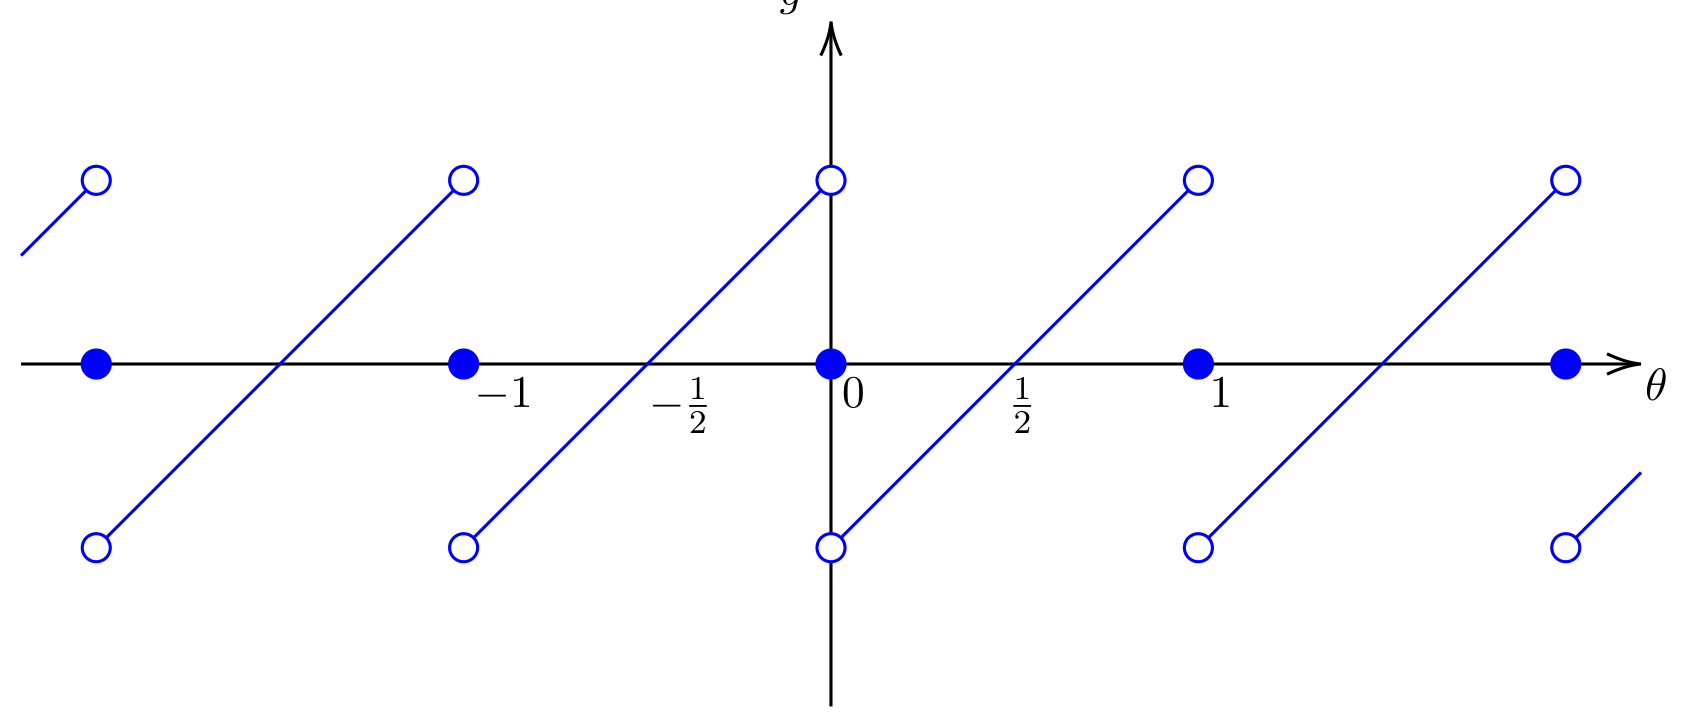
\includegraphics[width=0.40\textwidth]{figures/fig_p153_a.png}
\end{center}
% [图：原书 p.152]

\begin{proof}
  设 $g(\theta)$ 为上述周期函数。可计算它的傅里叶展开
  \[
  \begin{aligned}
  \int_0^1\ee^{-2\pi\ii n\theta}\Bigl(\theta-\frac12\Bigr)\rd\theta
  &\overset{(n\ne0)}{=}
  \frac{\ii}{2\pi n}\ee^{-2\pi\ii n\theta}\Bigl(\theta-\frac12\Bigr)\Big|_0^1
  -\int_0^1\ee^{-2\pi\ii n\theta}\rd\theta\\
  &=\frac{\ii}{2\pi n}.
  \end{aligned}
  \]
  \tutornote{原文此步第二项略去了因子 $\ii/(2\pi n)$；该项积分为零，不影响结果。}
  对 $n=0$，有 $\displaystyle\int_0^1\Bigl(\theta-\frac12\Bigr)\rd\theta=0$。故
  \[
  \theta-\frac12=\sum_{n\in\Z\setminus\{0\}}\frac{\ii}{2\pi n}
  \ee^{2\pi\ii n\theta},\qquad 0<\theta<1,
  \]
  正是所需。
\end{proof}

% [原文 p.153]
也可直接验证分布等式
\[
\frac{\pa}{\pa\theta_1}G(\theta_1,\theta_2)
=\hat\delta(\theta_1,\theta_2)=\delta(\theta_1,\theta_2)-1.
\]
对 $S^1$ 上任意光滑检验函数 $f(\theta)$，有
\[
\begin{aligned}
-\int_{S^1}G(\theta_1,\theta_2)f'(\theta_1)\rd\theta_1
&=-\int_{\theta_2-1}^{\theta_2}g(\theta_2-\theta_1)f'(\theta_1)\rd\theta_1\\
&=-\int_{\theta_2-1}^{\theta_2}\Bigl(\theta_2-\theta_1-\frac12\Bigr)f'(\theta_1)\rd\theta_1\\
&=-\Bigl(\theta_2-\theta_1-\frac12\Bigr)f(\theta_1)\Big|_{\theta_2-1}^{\theta_2}
-\int_{\theta_2-1}^{\theta_2}f(\theta_1)\rd\theta_1\\
&=f(\theta_2)-\int_{S^1}f(\theta)\rd\theta
=\int_0^1\bigl(\delta(\theta_1,\theta_2)-1\bigr)f(\theta_1)\rd\theta_1,
\end{aligned}
\]
正是所需。

于是得到两点函数
\[
\bigl\langle\mathbb X^k(\theta_1)\mathbb P_j(\theta_2)\bigr\rangle_\gamma^{S^1}
=\ii\hs G(\theta_1,\theta_2)\delta^k_j
=\ii\hs g(\theta_2-\theta_1)\delta^k_j.
\]
注意在极限 $\theta_1\to\theta_2$ 下
\[
\lim_{\theta_1\to\theta_2^-}\bigl\langle\mathbb X^k(\theta_1)\mathbb P_j(\theta_2)\bigr\rangle_\gamma^{S^1}
=-\frac{\ii\hs}{2}\delta^k_j,\qquad
\lim_{\theta_1\to\theta_2^+}\bigl\langle\mathbb X^k(\theta_1)\mathbb P_j(\theta_2)\bigr\rangle_\gamma^{S^1}
=\frac{\ii\hs}{2}\delta^k_j.
\]
故 $\theta_1$ 与 $\theta_2$ 彼此接近时，该两点函数化为 $\R$ 上的两点函数。这与预期相符，因为 $S^1$ 上的局部几何正是 $\R$。

\subsubsection*{$S^1$ 关联}

设 $A=\R[x^i,p_i]$ 为相空间上的多项式函数环。回忆有自然乘法映射
\[
A\otimes A\otimes\cdots\otimes A\longrightarrow A,\qquad
f_0\otimes f_1\otimes\cdots\otimes f_m\longmapsto f_0f_1\cdots f_m.
\]
作为 $S^1$ 量子力学模型的一个应用，我们构造上述乘法映射的量子化版本
$\langle f_0\otimes f_1\otimes\cdots\otimes f_m\rangle_{S^1}$，使
\[
\langle f_0\otimes f_1\otimes\cdots\otimes f_m\rangle_{S^1}
=f_0f_1\cdots f_m+O(\hs).
\]
令
\[
\mathrm{Cyc}_{m+1}(S^1)
=\Bigl\{(\theta_0,\theta_1,\cdots,\theta_m)\in(S^1)^{m+1}
\ \Big|\ \substack{\theta_0,\theta_1,\cdots,\theta_m\text{ 按顺时针}\\
\text{循环顺序互不相同}}\Bigr\}.
\]
\begin{center}
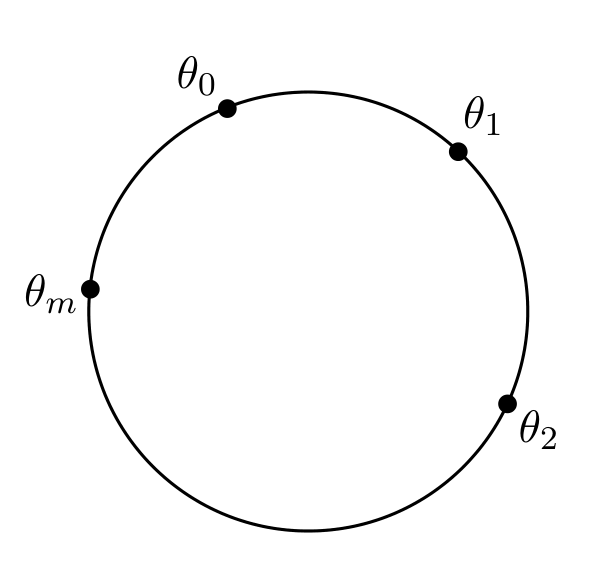
\includegraphics[width=0.40\textwidth]{figures/fig_p155_a.png}
\end{center}
% [图：原书 p.154]

% [原文 p.154]
利用旋转不变性，有
\[
\int_{\mathrm{Cyc}_{m+1}(S^1)}\rd\theta_0\rd\theta_1\cdots\rd\theta_m
=\int_{1\ge\theta_1\ge\cdots\ge\theta_m\ge0}\rd\theta_1\cdots\rd\theta_m
=\frac1{m!}.
\]

\begin{definition}{2.8.12}
  设 $f_i\in A$。定义它们的 $S^1$ 关联
  $\langle f_0\otimes f_1\otimes\cdots\otimes f_m\rangle_{S^1}\in A[\hs]$ 为
  \[
  \begin{aligned}
  &\langle f_0\otimes f_1\otimes\cdots\otimes f_m\rangle_{S^1}(\mathbf x,\mathbf p)\\
  &\quad=m!\int_{\mathrm{Cyc}_{m+1}(S^1)}\rd\theta_0\rd\theta_1\cdots\rd\theta_m
  \bigl\langle f_0(\mathbf x+\mathbb X(\theta_0),\mathbf p+\mathbb P(\theta_0))\cdots\\
  &\qquad\qquad\cdots f_m(\mathbf x+\mathbb X(\theta_m),\mathbf p+\mathbb P(\theta_m))
  \bigr\rangle_\gamma^{S^1}.
  \end{aligned}
  \]
  这里关联 $\langle-\rangle_\gamma^{S^1}$ 由 威克定理与费曼图定义。显式地
  \[
  \begin{aligned}
  &\bigl\langle f_0(\mathbf x+\mathbb X(\theta_0),\mathbf p+\mathbb P(\theta_0))
  \cdots f_m(\mathbf x+\mathbb X(\theta_m),\mathbf p+\mathbb P(\theta_m))\bigr\rangle_\gamma^{S^1}\\
  &\quad:=\ee^{\ii\hs\sum_{i,j=0}^mG(\theta_i,\theta_j)
  \frac{\pa}{\pa\mathbf x^{(i)}}\frac{\pa}{\pa\mathbf p^{(j)}}}
  f_0(\mathbf x^{(0)},\mathbf p^{(0)})\cdots f_m(\mathbf x^{(m)},\mathbf p^{(m)})
  \Big|_{\substack{\mathbf x^{(0)}=\cdots=\mathbf x^{(m)}=\mathbf x\\
  \mathbf p^{(0)}=\cdots=\mathbf p^{(m)}=\mathbf p}}.
  \end{aligned}
  \]
\end{definition}

显然
\[
\lim_{\hs\to0}\langle f_0\otimes f_1\otimes\cdots\otimes f_m\rangle_{S^1}
=f_0f_1\cdots f_m\,m!\int_{\mathrm{Cyc}_{m+1}(S^1)}\rd\theta_0\rd\theta_1\cdots\rd\theta_m
=f_0f_1\cdots f_m,
\]
它对应没有传播子的项。由于 $f_i$ 是多项式，只有有限个传播子会出现。于是
\[
A\otimes A\otimes\cdots\otimes A
\xrightarrow{\ \langle-\rangle_{S^1}\ }A[\hs].
\]

% [原文 p.155]
\begin{example}{2.8.13}
  给定两个多项式 $f_0,f_1\in A=\R[x,p]$，
  \begin{align*}
  \langle f_0\otimes f_1\rangle_{S^1}
  &=\int_{\mathrm{Cyc}_2(S^1)}\rd\theta_0\rd\theta_1\,f_0(x,p)\,
  \ee^{\ii\hs G(\theta_0,\theta_1)\overleftarrow{\frac{\pa}{\pa x}}
  \overrightarrow{\frac{\pa}{\pa p}}
  +\ii\hs G(\theta_1,\theta_0)\overleftarrow{\frac{\pa}{\pa p}}
  \overrightarrow{\frac{\pa}{\pa x}}}f_1(x,p)\\
  &=\int_0^1\rd\theta\,f_0(x,p)\,
  \ee^{\ii\hs g(\theta)\bigl(\overleftarrow{\pa_x}\overrightarrow{\pa_p}
  -\overleftarrow{\pa_p}\overrightarrow{\pa_x}\bigr)}f_1(x,p)\\
  &=\int_0^1\rd\theta\,f_0(x,p)\,
  \ee^{\ii\hs(\theta-\frac12)\bigl(\overleftarrow{\pa_x}\overrightarrow{\pa_p}
  -\overleftarrow{\pa_p}\overrightarrow{\pa_x}\bigr)}f_1(x,p)\\
  &=\int_{-\frac12}^{\frac12}\rd\theta\,f_0(x,p)\,
  \ee^{\ii\hs\theta\bigl(\overleftarrow{\pa_x}\overrightarrow{\pa_p}
  -\overleftarrow{\pa_p}\overrightarrow{\pa_x}\bigr)}f_1(x,p)\\
  &=\sum_{m=0}^\infty\int_{-\frac12}^{\frac12}\theta^{2m}\rd\theta\,
  \frac{(\ii\hs)^{2m}}{(2m)!}f_0(x,p)
  \bigl(\overleftarrow{\pa_x}\overrightarrow{\pa_p}
  -\overleftarrow{\pa_p}\overrightarrow{\pa_x}\bigr)^{2m}f_1(x,p)\\
  &=\sum_{m=0}^\infty\frac{(\ii\hs)^{2m}}{(2m+1)2^{2m}(2m)!}f_0(x,p)
  \bigl(\overleftarrow{\pa_x}\overrightarrow{\pa_p}
  -\overleftarrow{\pa_p}\overrightarrow{\pa_x}\bigr)^{2m}f_1(x,p).
  \end{align*}
  例如
  \[
  \langle x\otimes p\rangle_{S^1}=xp,\qquad
  \bigl\langle x^2\otimes p^2\bigr\rangle_{S^1}=x^2p^2-\frac{\hs^2}{6}.
  \]
\end{example}

\begin{example}{2.8.14}
  用 威克定理计算
  \begin{align*}
  \langle x\otimes xp\otimes p\rangle_{S^1}
  &=x^2p^2+2!\int_{\mathrm{Cyc}_3(S^1)}\rd\theta_0\rd\theta_1\rd\theta_2\\
  &\qquad\times\ii\hs\bigl(G(\theta_0,\theta_1)+G(\theta_1,\theta_2)+G(\theta_0,\theta_2)\bigr)xp\\
  &\quad+2!\int_{\mathrm{Cyc}_3(S^1)}\rd\theta_0\rd\theta_1\rd\theta_2\,(\ii\hs)^2
  G(\theta_0,\theta_1)G(\theta_1,\theta_2)\\
  &=x^2p^2+2xp(\ii\hs)\int_{1\ge\theta_1\ge\theta_2\ge0}\rd\theta_1\rd\theta_2\\
  &\qquad\times\bigl(G(1,\theta_1)+G(\theta_1,\theta_2)+G(1,\theta_2)\bigr)\\
  &\quad+2(\ii\hs)^2\int_{1\ge\theta_1\ge\theta_2\ge0}\rd\theta_1\rd\theta_2\,
  G(1,\theta_1)G(\theta_1,\theta_2)\\
  &=x^2p^2+2(\ii\hs)xp\int_{1\ge\theta_1\ge\theta_2\ge0}\rd\theta_1\rd\theta_2\\
  &\qquad\times\Bigl[\Bigl(\theta_1-\frac12\Bigr)-\Bigl((\theta_1-\theta_2)-\frac12\Bigr)
  +\Bigl(\theta_2-\frac12\Bigr)\Bigr]\\
  &\quad+2(\ii\hs)^2\int_{1\ge\theta_1\ge\theta_2\ge0}\rd\theta_1\rd\theta_2\,
  \Bigl(\theta_1-\frac12\Bigr)\Bigl(\frac12-(\theta_1-\theta_2)\Bigr)\\
  &=x^2p^2+\frac{\ii\hs}{6}xp.
  \end{align*}
\end{example}

\subsection{霍赫希尔德同调}

作为 $S^1$ 关联函数（定义 2.8.12）的一个应用，下面说明 $S^1$ 的几何如何与霍赫希尔德同调的概念相关联，并给出霍赫希尔德–科斯坦特–罗森伯格（Hochschild–Kostant–Rosenberg，HKR）映射的量子版本的一个显式构造。§6.4 将用这个量子 HKR 映射构造形变量子化中的迹映射。

% [原文 p.156]
\subsubsection*{霍赫希尔德同调}

设 $A$ 是基域 $k$ 上的结合代数。可定义链复形
\[
\cdots\xrightarrow{b}C_p(A)\xrightarrow{b}C_{p-1}(A)\xrightarrow{b}\cdots
\xrightarrow{b}C_1(A)\xrightarrow{b}C_0(A),
\]
其中
\[
C_p(A)=A^{\otimes p+1},
\]
这里 $\otimes=\otimes_k$。映射 $b$ 定义为
\[
\begin{aligned}
b(a_0\otimes a_1\otimes\cdots\otimes a_p)
&=a_0a_1\otimes a_2\otimes\cdots\otimes a_p
-a_0\otimes a_1a_2\otimes\cdots\otimes a_p\\
&\quad+\cdots+(-1)^{p-1}a_0\otimes a_1\otimes\cdots\otimes a_{p-1}a_p\\
&\quad+(-1)^pa_pa_0\otimes a_1\otimes\cdots\otimes a_{p-1}.
\end{aligned}
\]
\begin{center}
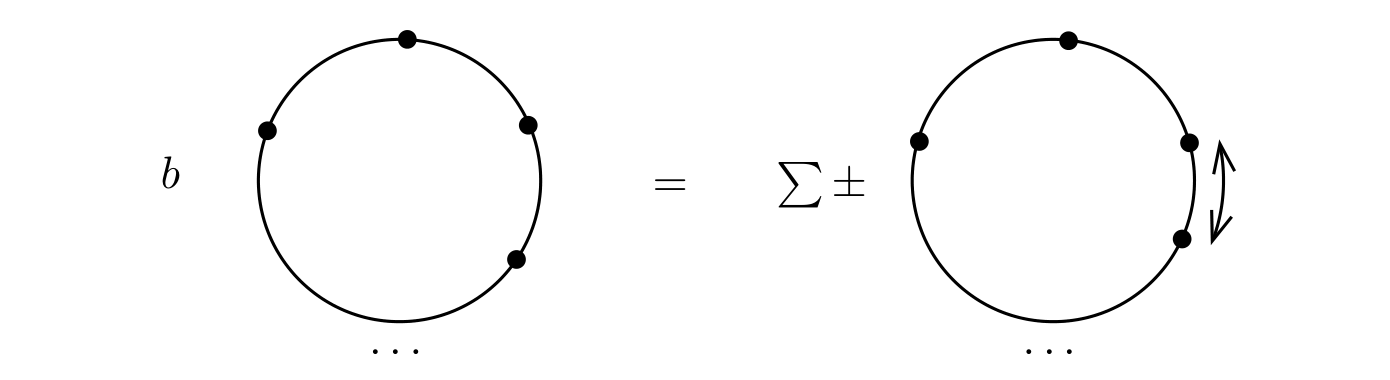
\includegraphics[width=0.62\textwidth]{figures/fig_p157_bop.png}
\end{center}
% [图：原书 p.156]

\underline{验证}：$b^2=0$。
\[
\begin{aligned}
b^2(a_0\otimes a_1\otimes\cdots\otimes a_p)
&=b\bigl(a_0a_1\otimes a_2\otimes\cdots\otimes a_p
-a_0\otimes a_1a_2\otimes\cdots\otimes a_p\pm\cdots\bigr)\\
&=(a_0a_1)a_2\otimes\cdots\otimes a_p-a_0(a_1a_2)\otimes\cdots\otimes a_p\pm\cdots\\
&=0,
\end{aligned}
\]
这里用到结合性。

链复形 $(C_\bullet(A),b)$ 称为\emph{霍赫希尔德链复形}（Hochschild chain complex），而
\[
HH_\bullet(A):=H_\bullet\bigl(C_\bullet(A),b\bigr)
\]
称为\emph{霍赫希尔德同调}（Hochschild homology）。

\begin{example}{2.8.15}
  \[
  C_2(A)\longrightarrow C_1(A)\xrightarrow{\ b\ }C_0(A),\qquad
  a_0\otimes a_1\longmapsto a_0a_1-a_1a_0.
  \]
  故 $HH_0(A)=A/[A,A]$ 是交换化。
\end{example}

\begin{theorem}{2.8.16}（霍赫希尔德–科斯坦特–罗森伯格（HKR））
  设 $A=k[y^i]$ 为多项式环，$\Omega^\bullet_A=k[y^i,\rd y^i]$ 为代数微分形式。则
  \[
  HH_p(A)=\Omega^p_A.
  \]
\end{theorem}

\begin{remark}{2.8.17}
  HKR 定理说的是：在标准交换空间 $k^n$ 上，
  \[
  HH_\bullet=\text{微分形式}.
  \]
  一般地，对结合但非交换的代数 $A$，可视为
  \[
  HH_\bullet=\text{非交换微分形式},
  \]
  这是在非交换世界做微积分的基本代数工具。
\end{remark}

% [原文 p.157]
HKR 同构由下式实现
\[
\rho:C_\bullet(A)\longrightarrow\Omega^\bullet_A,\qquad
f_0\otimes f_1\otimes\cdots\otimes f_p
\longmapsto f_0\rd f_1\wedge\rd f_2\wedge\cdots\wedge\rd f_p.
\]

\underline{验证}：$\rho(b(-))=0$。
\[
\begin{aligned}
\rho\bigl(b(f_0\otimes f_1\otimes\cdots\otimes f_p)\bigr)
&=\rho\bigl(f_0f_1\otimes f_2\otimes\cdots\otimes f_p
-f_0\otimes f_1f_2\otimes\cdots\otimes f_p\pm\cdots\bigr)\\
&=f_0f_1\rd f_2\wedge\cdots\wedge\rd f_p
-f_0\rd(f_1f_2)\wedge\rd f_3\wedge\cdots\wedge\rd f_p\pm\cdots\\
&\quad+(-1)^{p-1}f_0\rd f_1\wedge\cdots\wedge\rd(f_{p-1}f_p)\\
&\quad+(-1)^pf_pf_0\rd f_1\wedge\cdots\wedge\rd f_{p-1}\\
&=0.
\end{aligned}
\]
故 $\rho$ 定义了链复形的映射
\[
\rho:\bigl(C_\bullet(A),b\bigr)\longrightarrow\bigl(\Omega^\bullet_A,0\bigr).
\]
HKR 的更精确说法是：HKR 映射 $\rho$ 是拟同构，过到同调即诱导同构
\[
\rho:HH_\bullet(A)\xrightarrow{\ \simeq\ }\Omega^\bullet_A.
\]

\subsubsection*{量子 HKR}

设 $A=\C[x^i,p_i]$ 为相空间 $\R^{2n}$ 上的多项式函数环。$A$ 有标准的量子化，成为结合外尔代数
\[
A^\hs:=(A[\hs],*),
\]
其中 $*$ 为 Moyal 乘积。我们要描述 HKR 映射 $\rho$ 的量子版本 $\rho^\hs$，它与外尔代数 $A^\hs$ 的霍赫希尔德链复形 $C_\bullet(A^\hs)$ 相容。

设 $f_0,f_1,\cdots,f_m\in A$。回忆定义 2.8.12 给出的 $S^1$ 关联
$\langle f_0\otimes f_1\otimes\cdots\otimes f_m\rangle_{S^1}\in A[\hs]$。为简化记号，记
\[
\mathcal O_f(\theta):=f\bigl(\mathbf x+\mathbb X(\theta),\mathbf p+\mathbb P(\theta)\bigr),
\qquad \theta\in S^1.
\]
按构造
\[
\begin{aligned}
\langle f_0\otimes f_1\otimes\cdots\otimes f_m\rangle_{S^1}
&=m!\int_{\mathrm{Cyc}_{m+1}(S^1)}\rd\theta_0\rd\theta_1\cdots\rd\theta_m\\
&\qquad\times\bigl\langle\mathcal O_{f_0}(\theta_0)\mathcal O_{f_1}(\theta_1)\cdots
\mathcal O_{f_m}(\theta_m)\bigr\rangle_\gamma^{S^1}.
\end{aligned}
\]
给定 $f$，其全微分为
\[
\rd f=\sum_i\Bigl(\frac{\pa f}{\pa x^i}\rd x^i
+\frac{\pa f}{\pa p_i}\rd p_i\Bigr).
\]
记
\[
\mathcal O_{\rd f}(\theta):=\sum_i\Bigl(
\mathcal O_{\pa_{x^i}f}(\theta)\rd x^i
+\mathcal O_{\pa_{p_i}f}(\theta)\rd p_i\Bigr).
\]

% [原文 p.158]
\begin{definition}{2.8.18}
  定义\emph{量子 HKR 映射}（quantum HKR map）
  $\rho^\hs:A^{\otimes m+1}\to\Omega^m_A[\hs]$ 为
  \[
  \rho^\hs(f_0\otimes f_1\otimes\cdots\otimes f_m)
  :=\int_{\mathrm{Cyc}_{m+1}(S^1)}\rd\theta_0\rd\theta_1\cdots\rd\theta_m
  \bigl\langle\mathcal O_{f_0}(\theta_0)\mathcal O_{\rd f_1}(\theta_1)\cdots
  \mathcal O_{\rd f_m}(\theta_m)\bigr\rangle_\gamma^{S^1}.
  \]
  这可形式地写成
  \[
  \rho^\hs(f_0\otimes f_1\otimes\cdots\otimes f_m)
  =\frac1{m!}\langle f_0\otimes\rd f_1\otimes\cdots\otimes\rd f_m\rangle_{S^1}.
  \]
  用 威克定理，有显式公式
  \[
  \begin{aligned}
  &\rho^\hs(f_0\otimes f_1\otimes\cdots\otimes f_m)\\
  &\quad=\int_{\mathrm{Cyc}_{m+1}(S^1)}\rd\theta_0\rd\theta_1\cdots\rd\theta_m\,
  \ee^{\ii\hs\sum_{i,j=0}^mG(\theta_i,\theta_j)
  \frac{\pa}{\pa\mathbf x^{(i)}}\frac{\pa}{\pa\mathbf p^{(j)}}}\\
  &\qquad\times f_0(\mathbf x^{(0)},\mathbf p^{(0)})
  \rd f_1(\mathbf x^{(1)},\mathbf p^{(1)})\cdots\\
  &\qquad\qquad\cdots\rd f_m(\mathbf x^{(m)},\mathbf p^{(m)})
  \Big|_{\substack{\mathbf x^{(0)}=\cdots=\mathbf x^{(m)}=\mathbf x\\
  \mathbf p^{(0)}=\cdots=\mathbf p^{(m)}=\mathbf p}}.
  \end{aligned}
  \]
\end{definition}

接下来考察 $\rho^\hs$ 的代数结构。考虑如下积分
\[
\begin{aligned}
&\int_{\mathrm{Cyc}_{m+1}(S^1)}\rd\theta_0\rd\theta_1\cdots\rd\theta_m
\Bigl\{\frac{\pa}{\pa\theta_1}
\bigl\langle\mathcal O_{f_0}(\theta_0)\mathcal O_{f_1}(\theta_1)\cdots
\mathcal O_{\rd f_m}(\theta_m)\bigr\rangle_\gamma^{S^1}\\
&\qquad-\frac{\pa}{\pa\theta_2}
\bigl\langle\mathcal O_{f_0}(\theta_0)\mathcal O_{\rd f_1}(\theta_1)
\mathcal O_{f_2}(\theta_2)\cdots\mathcal O_{\rd f_m}(\theta_m)\bigr\rangle_\gamma^{S^1}\\
&\qquad+\cdots+(-1)^{m-1}\frac{\pa}{\pa\theta_m}
\bigl\langle\mathcal O_{f_0}(\theta_0)\mathcal O_{\rd f_1}(\theta_1)\cdots
\mathcal O_{\rd f_{m-1}}(\theta_{m-1})\mathcal O_{f_m}(\theta_m)\bigr\rangle_\gamma^{S^1}
\Bigr\}.
\end{aligned}
\tag*{$(\dagger)$}
\]
我们用两种方式计算式 $(\dagger)$。第一种是把 $\displaystyle\int\rd\theta_k
\frac{\pa}{\pa\theta_k}(-)$ 当作全导数来计算。由循环顺序
\begin{center}
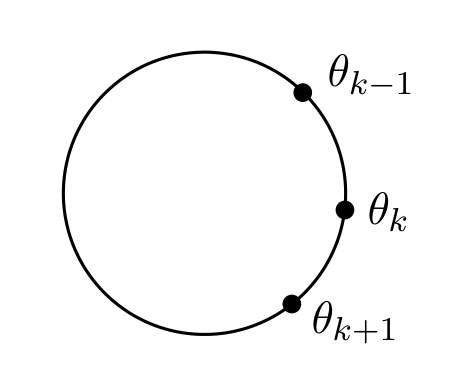
\includegraphics[width=0.22\textwidth]{figures/fig_p159_a.png}
\end{center}
% [图：原书 p.158]
有
\[
\int\rd\theta_k\frac{\pa}{\pa\theta_k}(-)
=\int_{\theta_{k+1}}^{\theta_{k-1}}\rd\theta_k\frac{\pa}{\pa\theta_k}(-)
=(-)\Big|_{\theta_{k+1}}^{\theta_{k-1}}.
\]
由 威克定理与 $S^1$ 传播子的性质，得到极限行为
\[
\begin{aligned}
\lim_{\theta_k\to\theta_{k-1}^-}
\bigl\langle\cdots\mathcal O_f(\theta_{k-1})\mathcal O_g(\theta_k)
\cdots\bigr\rangle_\gamma^{S^1}
&=\bigl\langle\cdots\mathcal O_{f*g}(\theta_{k-1})\cdots\bigr\rangle_\gamma^{S^1},\\
\lim_{\theta_k\to\theta_{k+1}^+}
\bigl\langle\cdots\mathcal O_f(\theta_k)\mathcal O_g(\theta_{k+1})
\cdots\bigr\rangle_\gamma^{S^1}
&=\bigl\langle\cdots\mathcal O_{f*g}(\theta_{k+1})\cdots\bigr\rangle_\gamma^{S^1}.
\end{aligned}
\]

% [原文 p.159]
于是按全导数计算式 $(\dagger)$ 得到
\[
\begin{aligned}
&\frac1{(m-1)!}\langle f_0*f_1\otimes\rd f_2\otimes\cdots\otimes\rd f_m\rangle_{S^1}\\
&\quad-\frac1{(m-1)!}\langle f_0\otimes f_1*\rd f_2\otimes\cdots\otimes\rd f_m\rangle_{S^1}\\
&\quad-\frac1{(m-1)!}\langle f_0\otimes\rd f_1*f_2\otimes\rd f_3\otimes\cdots\otimes\rd f_m\rangle_{S^1}\\
&\quad+\frac1{(m-1)!}\langle f_0\otimes\rd f_1\otimes f_2*\rd f_3\otimes\cdots\otimes\rd f_m\rangle_{S^1}\\
&\quad+\cdots+(-1)^{m-1}\frac1{(m-1)!}
\langle f_0\otimes\rd f_1\otimes\cdots\otimes\rd f_{m-1}*f_m\rangle_{S^1}\\
&\quad-(-1)^{m-1}\frac1{(m-1)!}
\langle f_m*f_0\otimes\rd f_1\otimes\cdots\otimes\rd f_{m-1}\rangle_{S^1}.
\end{aligned}
\]
由 Moyal 乘积的公式，有
\[
\rd(f*g)=\rd f*g+f*\rd g,
\]
其中
\[
\begin{aligned}
\rd f*g&=\sum_i\bigl((\pa_{x^i}f*g)\rd x^i+(\pa_{p_i}f*g)\rd p_i\bigr),\\
f*\rd g&=\sum_i\bigl((f*\pa_{x^i}g)\rd x^i+(f*\pa_{p_i}g)\rd p_i\bigr).
\end{aligned}
\]
于是式 $(\dagger)$ 变为
\[
\begin{aligned}
&\frac1{(m-1)!}\langle f_0*f_1\otimes\rd f_2\otimes\cdots\otimes\rd f_m\rangle_{S^1}\\
&\quad-\frac1{(m-1)!}\langle f_0\otimes\rd(f_1*f_2)\otimes\cdots\otimes\rd f_m\rangle_{S^1}\\
&\quad+\cdots+(-1)^{m-1}\frac1{(m-1)!}
\langle f_0\otimes\rd f_1\otimes\cdots\otimes\rd(f_{m-1}*f_m)\rangle_{S^1}\\
&\quad+(-1)^m\frac1{(m-1)!}
\langle f_m*f_0\otimes\rd f_1\otimes\cdots\otimes\rd f_{m-1}\rangle_{S^1}\\
&=\rho^\hs\bigl(b(f_0\otimes f_1\otimes\cdots\otimes f_m)\bigr).
\end{aligned}
\]
这里 $b$ 是关于 Moyal 乘积的霍赫希尔德微分。

计算式 $(\dagger)$ 的第二种方式是显式计算
$\displaystyle\frac{\pa}{\pa\theta_k}\langle\cdots\rangle_\gamma^{S^1}$。注意当 $\theta_j\ne\theta_k$ 时
\[
\frac{\pa}{\pa\theta_k}G(\theta_k,\theta_j)
=-1=-\frac{\pa}{\pa\theta_k}G(\theta_j,\theta_k).
\]
因此
\[
\begin{aligned}
&\frac{\pa}{\pa\theta_k}
\bigl\langle\mathcal O_{f_0}(\theta_0)\mathcal O_{\rd f_1}(\theta_1)\cdots
\mathcal O_{\rd f_{k-1}}(\theta_{k-1})\mathcal O_{f_k}(\theta_k)\cdots
\mathcal O_{\rd f_m}(\theta_m)\bigr\rangle_\gamma^{S^1}\\
&\quad=\ii\hs\sum_i\frac{\pa}{\pa x^i}
\bigl\langle\mathcal O_{f_0}(\theta_0)\mathcal O_{\rd f_1}(\theta_1)\cdots
\mathcal O_{\rd f_{k-1}}(\theta_{k-1})\mathcal O_{\pa_{p_i}f_k}(\theta_k)\cdots
\mathcal O_{\rd f_m}(\theta_m)\bigr\rangle_\gamma^{S^1}\\
&\qquad-\ii\hs\sum_i\frac{\pa}{\pa p_i}
\bigl\langle\mathcal O_{f_0}(\theta_0)\mathcal O_{\rd f_1}(\theta_1)\cdots
\mathcal O_{\rd f_{k-1}}(\theta_{k-1})\mathcal O_{\pa_{x^i}f_k}(\theta_k)\cdots
\mathcal O_{\rd f_m}(\theta_m)\bigr\rangle_\gamma^{S^1}.
\end{aligned}
\]
引入如下算子
\[
\Delta:\Omega^m_A\longrightarrow\Omega^{m-1}_A,\qquad
\Delta=\sum_i\Bigl(\frac{\pa}{\pa x^i}\iota_{\pa_{p_i}}
-\frac{\pa}{\pa p_i}\iota_{\pa_{x^i}}\Bigr).
\]

% [原文 p.160]
设 $\omega^{-1}=\sum_i\frac{\pa}{\pa x^i}\wedge\frac{\pa}{\pa p_i}$ 为泊松双向量。则 $\Delta$ 几何上就是李导数
\[
\Delta=\mathcal L_{\omega^{-1}}.
\]
显然 $\Delta^2=0$。$\Delta$ 是量子规范理论中 Batalin–Vilkovisky (BV) 算子的原型。于是上述计算给出
\[
(\dagger)=\ii\hs\Delta\rho^\hs(f_0\otimes f_1\otimes\cdots\otimes f_m).
\]
比较两种计算，得到
\[
\rho^\hs(b(-))=\ii\hs\Delta\bigl(\rho^\hs(-)\bigr),
\]
这里 $b$ 是关于 Moyal 乘积的霍赫希尔德微分。
\tutornote{原文此处把 $\rho^\hs$ 误写作 $\sigma^\hs$，译文统一写 $\rho^\hs$。}

可把 $\rho^\hs$ 沿 $\hs$ 线性延拓为
\[
\rho^\hs:C_\bullet(A^\hs)\longrightarrow\Omega^\bullet_A[\hs].
\]
于是上述计算表明 $\rho^\hs$ 是链复形的态射
\[
\rho^\hs:\bigl(C_\bullet(A^\hs),b\bigr)\longrightarrow
\bigl(\Omega^\bullet_A[\hs],\ii\hs\Delta\bigr).
\]
故 $\rho^\hs$ 给出 $\rho$ 的一个量子化。

\begin{remark}{2.8.19}
  还可进一步局部化 $\hs$，记
  \[
  A(\hs):=A^\hs\otimes_{k[\hs]}k[\hs,\hs^{-1}].
  \]
  量子 HKR 映射 $\rho^\hs$ 自然延拓为
  \[
  \rho^\hs:\bigl(C_\bullet(A(\hs)),b\bigr)\longrightarrow
  \bigl(\Omega^\bullet_A[\hs,\hs^{-1}],\ii\hs\Delta\bigr).
  \]
  $A(\hs)$ 的霍赫希尔德同调与 $\bigl(\Omega^\bullet_A[\hs,\hs^{-1}],\ii\hs\Delta\bigr)$ 的同调都集中在次数 $2n$。过到同调，$\rho^\hs$ 恰好给出 $HH_{2n}(A(\hs))$ 上的 Feigin–Felder–Shoikhet 迹公式~[21]。
\end{remark}

\takeaway{微扰展开把发散积分重定义为幂级数，用 威克定理逐项赋值，得到费曼图展开。两点函数由 $\rd/\rd t$ 的格林函数给出，时间轴上的插入复现 Moyal 乘积与结合性；$S^1$ 上的零模与周期性导出量子化乘法与量子 HKR 映射。}

\chapterreview{%
本章从量子演化的费曼核出发，把路径积分定义为时间切片上无穷维积分的极限，并在自由粒子、谐振子等可解模型上验证了它。高斯路径积分给出二次作用量的通用公式，zeta 函数正则化处理行列式。渐近方法、最速下降、莫尔斯流与斯托克斯现象说明半经典极限如何决定跃迁振幅的指数因子与前因子，半经典费曼核与雅可比场把图像落实到具体计算。格林函数在固定能量下把时间与能量互换，路径积分的 WKB 分析由此给出能级与隧穿的信息。最后，微扰展开用 威克定理与费曼图把发散积分组织为渐近级数，再把组合公式搬到相空间路径积分上，得到 Moyal 乘积与量子 HKR 映射，将路径积分、形变量子化与霍赫希尔德同调联系起来。}

